\documentclass[12pt,oneside]{book} % for one-sided printing

\usepackage{blindtext}% Just used so we can generate some example text
\usepackage{amsmath}
\usepackage{amssymb}
\usepackage{mathtools}
\usepackage[export]{adjustbox}
\usepackage{lipsum}
\usepackage{booktabs}  % For better quality tables
\usepackage{tabularx}  % for the X column type
\usepackage{listings}
\usepackage{xcolor}
\usepackage{caption}
\usepackage{xfrac}
\usepackage{algorithmic}
\usepackage{indentfirst}
\usepackage{subcaption}
\usepackage{graphicx}
\usepackage{geometry}
\geometry{a4paper, margin=1in}

% Place style file after other packages.
\usepackage{cranfieldthesis}
\usepackage{lscape} % for landscape pages
\usepackage{float}
\usepackage[toc,title,page]{appendix}

% Couleurs personnalisées
\definecolor{backcolour}{rgb}{0.96, 0.96, 0.96} % Fond très clair
\definecolor{codegray}{rgb}{0.47, 0.47, 0.47}   % Commentaires et numéros de ligne
\definecolor{codegreen}{rgb}{0.25, 0.50, 0.35}  % Commentaires
\definecolor{codeblue}{rgb}{0.26, 0.44, 0.58}   % Mots-clés
\definecolor{codepurple}{rgb}{0.50, 0, 0.50}    % Identificateurs
\definecolor{codeteal}{rgb}{0, 0.5, 0.5}        % Chaînes de caractères
\definecolor{terminalback}{rgb}{0.05, 0.05, 0.05} % Fond très sombre pour le terminal
\definecolor{terminaltext}{rgb}{0.7, 0.7, 0.7}    % Texte clair pour le terminal
\definecolor{mygreen}{rgb}{0,0.6,0}
\definecolor{mygray}{rgb}{0.5,0.5,0.5}
\definecolor{mymauve}{rgb}{0.58,0,0.82}
\definecolor{terminalbgcolor}{HTML}{330033}
\definecolor{terminalrulecolor}{HTML}{000099}

\lstdefinestyle{pythonstyle}{
    language=Python,
    backgroundcolor=\color{backcolour},
    commentstyle=\color{codegreen},
    keywordstyle=\color{codeblue},
    numberstyle=\tiny\color{codegray},
    stringstyle=\color{codeteal},
    identifierstyle=\color{codepurple},
    basicstyle=\ttfamily\scriptsize,
    breakatwhitespace=false,
    breaklines=true,
    captionpos=b,
    keepspaces=true,
    numbers=left,
    numbersep=5pt,
    showspaces=false,
    showstringspaces=false,
    showtabs=false,
    tabsize=4,
    frame=single,
    rulecolor=\color{codegray},
    framexleftmargin=15pt,
    framextopmargin=5pt,
    framexbottommargin=5pt,
    framexrightmargin=15pt,
}

\lstdefinestyle{bashstyle}{
    language=bash,
    backgroundcolor=\color{backcolour},
    basicstyle=\ttfamily\scriptsize,
    keywordstyle=\color{blue},
    stringstyle=\color{red},
    identifierstyle=\color{codepurple},
    commentstyle=\color{codegreen},
    morecomment=[l]{\#},   % Define comment style
    frame=single,          % adds a frame around the code
    rulecolor=\color{gray},% if not set, the frame-color may be changed on line-breaks
    breakatwhitespace=false,
    breaklines=true,       % sets automatic line breaking
    captionpos=b,          % sets the caption-position to bottom
    keepspaces=true,       % keeps spaces in text
    showspaces=false,      % show spaces everywhere adding particular underscores
    showstringspaces=false % underline spaces within strings only
}

\lstdefinestyle{ymlstyle}{
    language=Python,
    backgroundcolor=\color{backcolour},
    basicstyle=\ttfamily\scriptsize,
    keywordstyle=\color{blue},
    stringstyle=\color{red},
    identifierstyle=\color{codepurple},
    commentstyle=\color{codegreen},
    morecomment=[l]{\#},   % Define comment style
    frame=single,          % adds a frame around the code
    rulecolor=\color{gray},% if not set, the frame-color may be changed on line-breaks
    breakatwhitespace=false,
    breaklines=true,       % sets automatic line breaking
    captionpos=b,          % sets the caption-position to bottom
    keepspaces=true,       % keeps spaces in text
    showspaces=false,      % show spaces everywhere adding particular underscores
    showstringspaces=false, % underline spaces within strings only
    literate=% Special handling for dot notations
        {http.response_time.p99}{{\textcolor{blue}{http.response\_time.p99}}}{18}
        {http.response_time.p95}{{\textcolor{blue}{http.response\_time.p95}}}{18}
        {metrics-by-endpoint}{{\textcolor{blue}{metrics-by-endpoint}}}{16},
    morekeywords={config, flow, target, phases, plugins, scenarios, loop, get, url, count, ensure, apdex, threshold, thresholds, duration, arrivalRate, name, pause, metrics -by-endpoint}, % Additional YAML-specific keywords
}

\lstdefinestyle{servicestyle}{
backgroundcolor=\color{backcolour},      % choose the background color
basicstyle=\ttfamily\scriptsize, % print whole listing white
keywordstyle=\color{blue},          % attributes in blue
stringstyle=\color{red},            % values in red
identifierstyle=\color{codepurple},
breakatwhitespace=false,
breaklines=true,                    % sets automatic line breaking
captionpos=b,                       % sets the caption-position to bottom
keepspaces=true,                    % keeps spaces in text
showspaces=false,                   % show spaces everywhere adding particular underscores
showstringspaces=false,             % underline spaces within strings only
frame=single,                       % adds a frame around the code
rulecolor=\color{gray},             % if not set, the frame-color may be changed on line-breaks
morecomment=[l]{\#},                % Define comment style
moredelim=[s][\color{codegreen}]{[}{]}, % color everything between [ and ] in green
morekeywords={Description,Wants,After,ExecStart,WantedBy,EnvironmentFile,User,Group,Type,Restart,Documentation,WorkingDirectory,RuntimeDirectory,RuntimeDirectoryMode,LimitNOFILE,TimeoutStopSec,CapabilityBoundingSet,DeviceAllow,LockPersonality,MemoryDenyWriteExecute,NoNewPrivileges,PrivateDevices,PrivateTmp,ProtectClock,ProtectControlGroups,ProtectHome,ProtectHostname,ProtectKernelLogs,ProtectKernelModules,ProtectKernelTunables,ProtectProc,ProtectSystem,RemoveIPC,RestrictAddressFamilies,RestrictNamespaces,RestrictRealtime,RestrictSUIDSGID,SystemCallArchitectures,UMask} % add your attributes here
}

% Title Page Set Up
\title{Cloud Computing Assignment}
\author{Alexis Balayre}
\date{2\textsuperscript{nd} January 2024}
\school{\SATM}
\degree{MSc}
\course{Computational Software of Techniques Engineering}
\academicyear{2023 - 2024}

% Supervisors
\supervisor{Dr Stuart Barnes}

% Copyright
\copyrightyear{2024}

% References
\usepackage[numbers]{natbib} % for nice referencing
\makeatletter % Reference list option change to number and period
\renewcommand\@biblabel[1]{#1.} % from [1] to 1
\makeatother %
\setcitestyle{round} % use round citations

\begin{document}

\frontmatter

% Form Title Pages
\maketitle

% Use single spacing for Table of Contents, List of Figures, etc
{
    \clearpage
    \singlespacing
    % Table of Contents
    {
        \tableofcontents
    }
    \clearpage

    % List of Figures
    \listoffigures

    % List of Tables
    \listoftables
}

%% Main Matter
\mainmatter
\pagestyle{fancy}
\fancyhead[L]{\nouppercase{\leftmark}}
\fancyhead[R]{\nouppercase{\rightmark}}

\chapter{Introduction}
In an increasingly connected world, cloud computing and the Internet of Things
(IoT) are revolutionising many fields, including environmental monitoring. This
technological development offers unprecedented possibilities for managing and
analysing air quality, a major public health issue. This report, drawn up as
part of my Master's degree in Cloud and Embedded Systems Science and Technology
(CSTE), focuses on the use of these technologies to collect, process and
distribute environmental data.

The main aim of this assignment is to store and make accessible the latest air
quality data, captured by a network of small environmental IoT sensors. The
project aims to provide a reliable platform for real-time consultation of
environmental data, a crucial tool for researchers, decision-makers and the
general public.

We face a number of technical challenges in achieving this objective. Firstly,
managing the large quantities of data generated by IoT sensors requires a
robust and adaptable cloud infrastructure. Secondly, calculating the Air
Quality Index (AQI) from this data in real time requires considerable
processing power and accuracy. Finally, the need to keep the system adaptable
and responsive to varying workloads presents an additional challenge.

To address these challenges, our approach is to use a database located in the
cloud, specifically designed to manage and process large volumes of IoT data.
This database will be regularly updated with new data, while allowing quick and
easy access for end users. In addition, we will be implementing advanced
algorithms for calculating the AQI, guaranteeing the accuracy and reliability
of the information provided.

The importance of this system is not limited to environmental monitoring; it
also has a significant impact on public health, urban planning and
environmental awareness. By providing accurate and up-to-date data, we
contribute to a better understanding and management of air quality.

In conclusion, this report will detail our methodology, the architecture of the
system, the challenges encountered and the solutions adopted. We will also
discuss the implications of our work, not only in technical terms but also in
terms of its practical applications and impact on different stakeholders.

\chapter{Methodologies}\label{chap:one}

\section{Data Collecting, Processing \& Storing}

\subsection{Overview of the Pipeline Architecture}

The initial pipeline in this project consists of three primary components:
\textbf{Data Collecting}, \textbf{Data Processing}, and \textbf{Data Storing}.

During the \textbf{Data Collecting} phase, the most recent version of the
dataset is acquired from its source. This is followed by the \textbf{Data
    Processing} phase, where the data is formatted, and the Air Quality Index (AQI)
is calculated for each particulate matter sensor. Lastly, in the \textbf{Data
    Storing} phase, the data from each sensor is methodically stored in a
time-series database.

\begin{figure}[H]
    \centering
    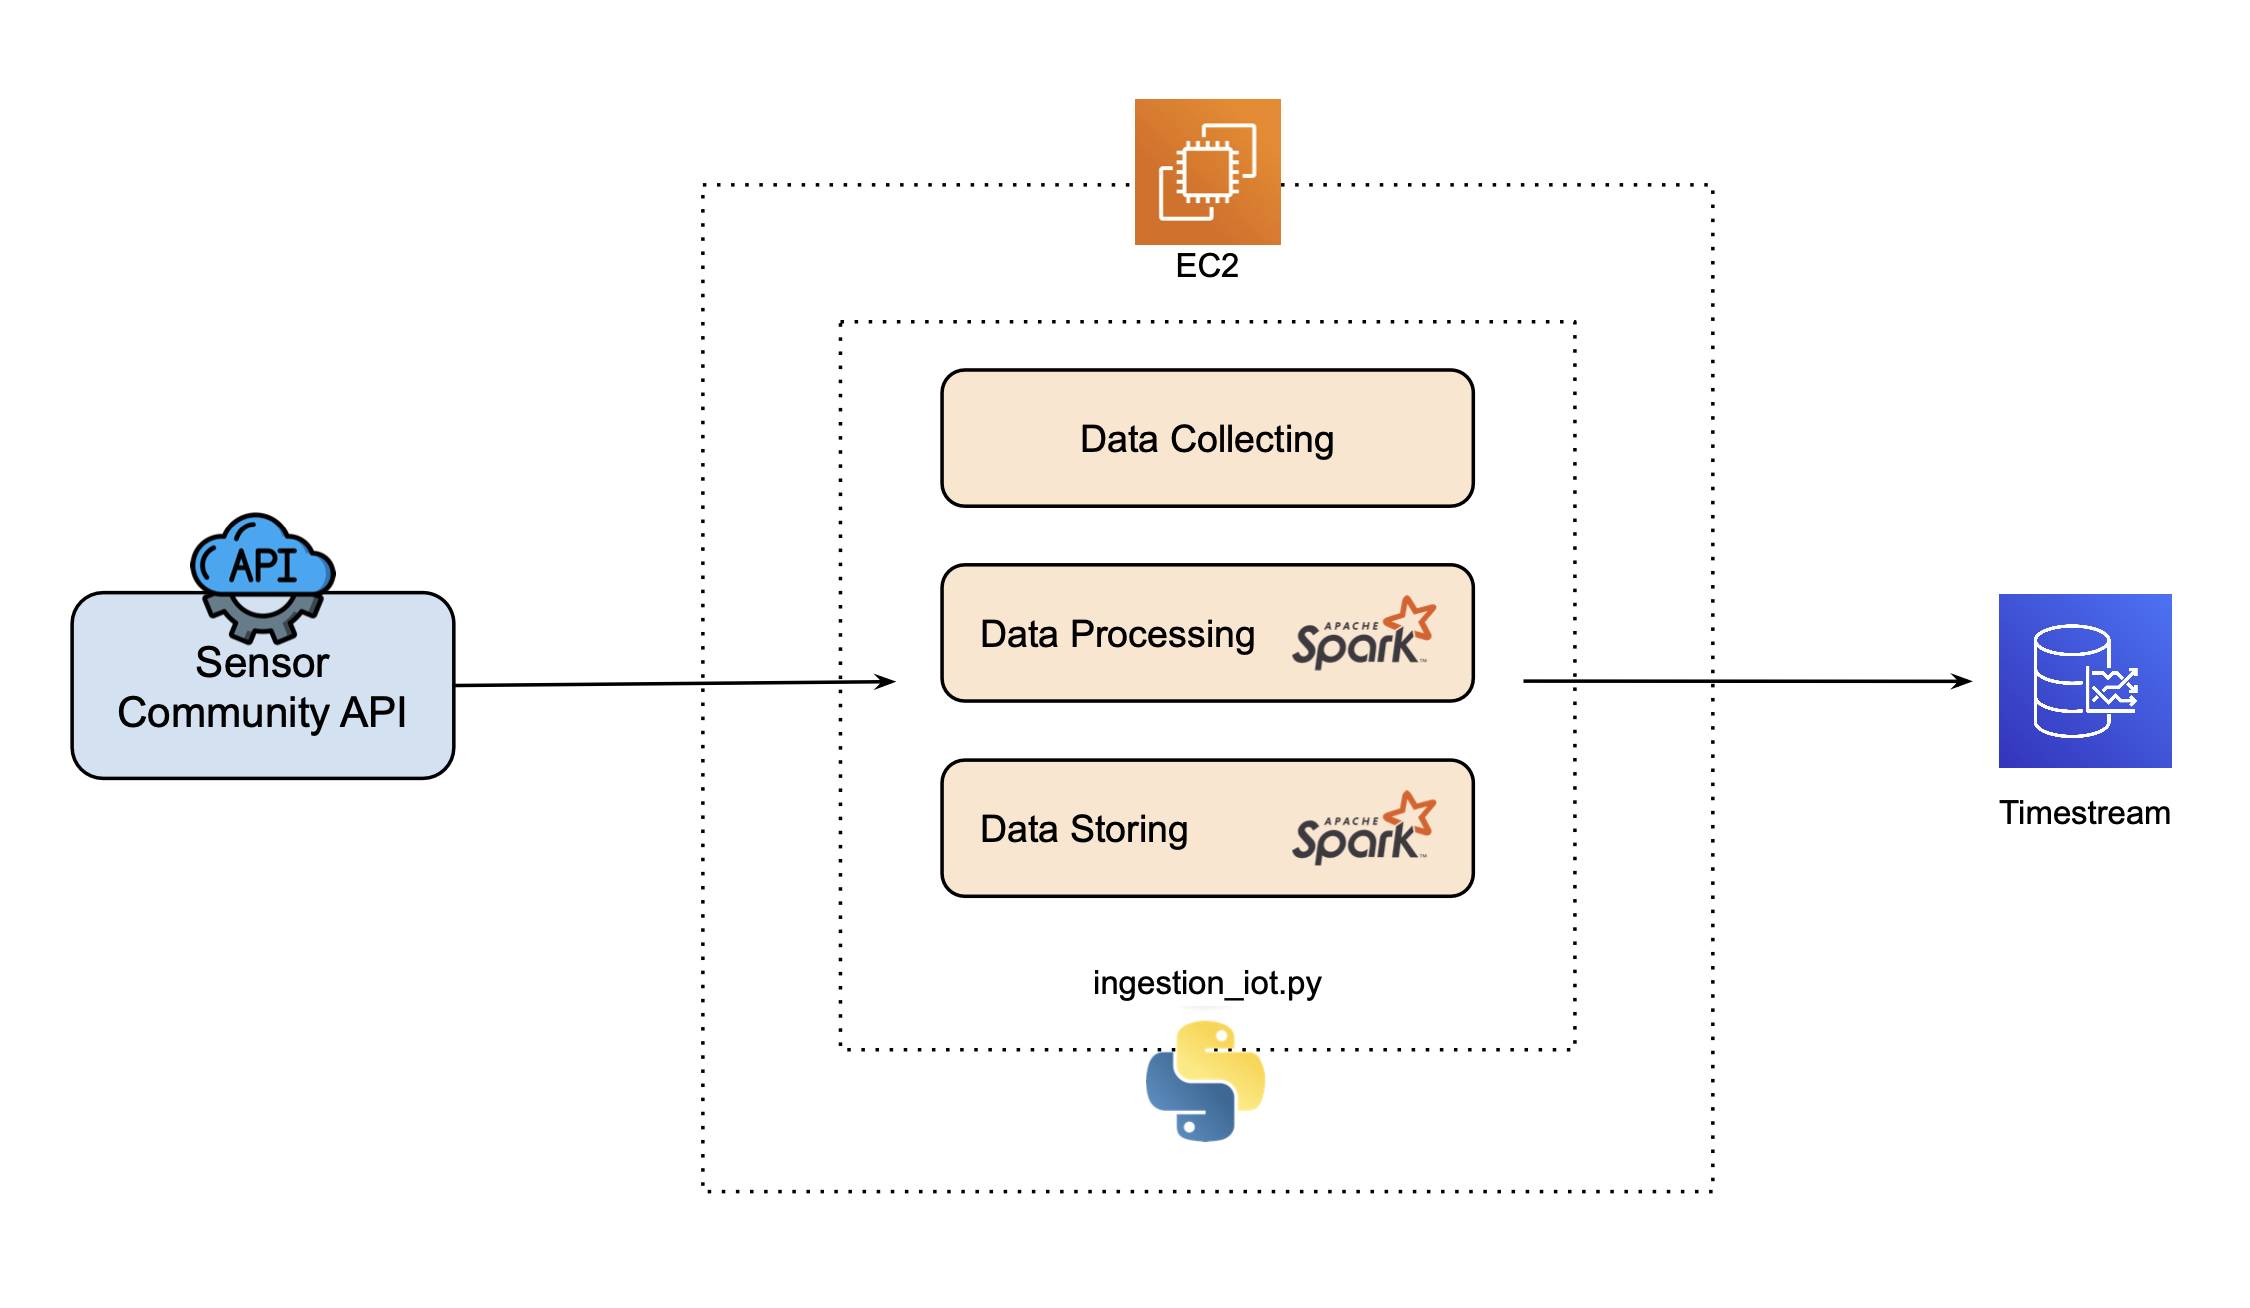
\includegraphics[width=1\linewidth]{images/cloud-computing-data-ingestion.png}
    \caption{Data Collecting, Processing \& Storing Pipeline Diagram}
\end{figure}

\subsection{Data Collecting}
\subsubsection{Data Source}
The Sensor Community network is a global, contributor-driven initiative that
collects open environmental data through a vast network of sensors. These
sensors, deployed in over 70 countries, collect real-time data on air quality,
temperature, humidity and pressure. On average, the sensors send new data every
145 seconds~\cite{sensorcommunity2023synchronization}. The Sensor Community
network offers two main API endpoints for accessing their environmental data:

\begin{enumerate}
    \item \textbf{5-Minute Averaged Data API:} This API provides data averaged over the last 5 minutes for each sensor. This is useful for near real-time analysis or immediate air quality assessments, particularly in test or active monitoring contexts.
    \item \textbf{24 Hour Averaged Data API:} This API provides data averaged over the last 24 hours for each sensor. It is particularly suited to analysing daily trends and understanding environmental changes over a longer period.
\end{enumerate}

\subsubsection{Ingestion Script}
The data acquisition process in this project involved leveraging both APIs from
the Sensor Community. To facilitate this, the Python \texttt{requests} library
was employed, enabling efficient data retrieval. Once collected, the data was
temporarily stored in a local cache, formatted as a Spark DataFrame for
optimized handling and processing. This operation, executed by the
\texttt{fetch\_sensors\_data} function, is located within the
\texttt{collecting.py} script (see Appendix~\ref{appendix:collecting} for
detailed code). Notably, this function is programmed to run at a consistent
interval of every 10 seconds, ensuring a steady and up-to-date flow of data
from the sensors. This systematic approach not only streamlines the data
collection process but also enhances the reliability and timeliness of the
gathered information.

\subsection{Data Processing}

\subsubsection{Processing Script}
Once the data has been ingested, the \texttt{computeAQI} function is called to
compute the Air Quality Index (AQI) values using user-defined functions (UDFs)
that transform measured PM2.5 and PM10 concentrations into the corresponding
AQI values, based on the thresholds as defined in Table~\ref{tab:uk_aqi}. This
operation, located within the \texttt{processing.py} script (see
Appendix~\ref{appendix:processing} for detailed code), utilises UDFs applied to
a Spark DataFrame, a distributed collection of data organised into named
columns, which facilitates data processing operations. The \texttt{explode}
operation on the DataFrame transforms the sensor data values into individual
rows, enabling the UDFs to be applied to each concentration measurement. The
process is optimised by caching the DataFrame, thereby reducing processing time
by minimising read and write operations to disk.

This procedure uses Apache Spark, a distributed data processing system, to
calculate the AQI from data collected in real time by sensors. Spark's
distributed approach is especially adept at managing the large volumes of data
generated by sensors, enabling the AQI to be calculated quickly and
efficiently.

Finally, the AQI is calculated by grouping the data by sensor ID and timestamp,
followed by aggregation to determine the maximum AQI value between PM2.5 and
PM10 particles. This ensures that the AQI reflects the highest concentration of
pollutants, which is essential for an accurate assessment of exposure to air
pollutants. This distributed calculation, performed in parallel across multiple
processing nodes, illustrates the power of Spark in processing environmental
IoT data, providing up-to-date and accurate air quality information that is
essential for public health decision-making.

\begin{table}[H]
    \centering
    \caption{UK air quality index, ``Review of the UK Air Quality Index'', 2011}
    \begin{tabular}{|p{2cm}|p{2cm}|p{3,5cm}|p{3,5cm}|}
        \hline
        \textbf{Range} & \textbf{Air Quality Index} & \textbf{PM\(_{2.5}\) Particles, 24 hour mean (\(\mu g/m^3\))} & \textbf{PM\(_{10}\) Particles, 24 hour mean (\(\mu g/m^3\))} \\ \hline
        Low            & 1                          & 0-11                                                          & 0-16                                                         \\
                       & 2                          & 12-23                                                         & 17-33                                                        \\
                       & 3                          & 24-35                                                         & 34-50                                                        \\ \hline
        Medium         & 4                          & 36-41                                                         & 51-58                                                        \\
                       & 5                          & 42-47                                                         & 59-66                                                        \\
                       & 6                          & 48-53                                                         & 67-75                                                        \\ \hline
        High           & 7                          & 54-58                                                         & 76-83                                                        \\
                       & 8                          & 59-64                                                         & 84-91                                                        \\
                       & 9                          & 65-70                                                         & 92-100                                                       \\ \hline
        Very High      & 10                         & $>$70                                                         & $>$100                                                       \\ \hline
    \end{tabular}
    \label{tab:uk_aqi}
\end{table}

\subsection{Data Storing}

\subsubsection{Database Choice}
The difficulty with this project lies in the efficient management of data
storage. Each sensor can measure a variety of data, making the structure of a
single relational database too complex and inefficient. This complexity
increases as the volume of data increases, requiring the creation of multiple
linked tables. This structural challenge poses a performance problem,
particularly when it comes to processing and analysing large quantities of data
in real time, a crucial aspect for applications such as air quality or
environmental monitoring.

Faced with these challenges, time series databases (TSDBs) are emerging as an
optimal solution. Unlike traditional relational databases, TSDBs are
specifically designed to manage time-series data, such as that from IoT
sensors. They offer better performance in tracking, monitoring and aggregating
data over time. In addition, TSDBs such as Amazon Timestream stand out for
their ability to ingest data quickly and process large volumes efficiently,
while ensuring regular updates and in-depth analysis, essential aspects for
applications such as Air Quality Index analysis.

Amazon Timestream is a good choice for this project. As a cloud-native
time-series database, it offers superior time-series management capabilities
tailored to IoT sensor data. What sets Amazon Timestream apart is the speed
with which it ingests data and its efficiency in processing large volumes of
data, enabling regular updates and in-depth analysis. Its ability to adapt to
changing workloads ensures consistent performance, a major advantage for
real-time data management. What's more, its advanced security features meet
strict standards of confidentiality and data sovereignty, an essential

\subsubsection{Storing Script}
The data storing process represents the final phase in the IoT data collecting
and processing pipeline. Once the Air Quality Index (AQI) has been calculated,
the data must be stored efficiently and securely to allow subsequent analysis
and real-time consultation. The \texttt{storing.py} script (see
Appendix~ref{appendix:storing} for detailed code) is designed to interact with
the Amazon Timestream database.

The \texttt{keepOnlyUpdatedRows} function is responsible for checking what data
is already in Timestream and keeping only the newly updated values. This
process begins by querying Timestream to retrieve the latest data timestamp for
each sensor using the `boto3` client. The data is then filtered to exclude
records that do not reflect new measurements, optimising storage space and
database performance.

Once this filtering is complete, the \texttt{writeToTimestream} function takes
over. It transforms each partition of the Spark DataFrame into a series of
structured records, containing the dimensions and measurements corresponding to
each sensor. These records are then written to Timestream in batches. The
process is carefully managed to ensure that records are written atomically and
consistently, with robust exception handling to deal with any rejected records.

In conclusion, the integration of Spark with Amazon Timestream offers a
powerful solution for storing environmental sensor data. Spark's ability to
process and filter data in a distributed manner aligns perfectly with
Timestream's high availability and auto-scaling capabilities, ensuring a
resilient, high-performance data infrastructure. This arrangement enables
reliable data storage and rapid retrieval, which are essential for continuous
monitoring of air quality and rapid responses to environmental issues.

\newpage
\subsection{Pipeline Implementation on AWS}
Setting up an IoT data processing pipeline on Amazon Web Services (AWS)
involves several key steps, from configuring the EC2 instance to running and
managing the pipeline. The process is described below:

\begin{enumerate}
    \item \textbf{EC2 Instance Configuration:} An EC2 t4g.small instance has been configured to host the data pipeline. A t4g.small instance was chosen for its balance between performance and energy efficiency. These instances, based on ARM architecture, are ideal for light to moderate workloads, which correspond to the requirements of continuous data processing. In addition, Apache Spark has been installed on this instance to process the data collected. Spark was chosen for its ability to process data in memory and in parallel, optimising performance for data processing workloads.
    \item \textbf{Setting Up Automated Services:} Two systemd services were then set up to automate the essential tasks: The \texttt{get\_iam\_credentials.service} (see Appendix~\ref{appendix:get-iam-credentials-service}) executes \texttt{get\_iam\_credentials.sh} (see Appendix~\ref{appendix:get-iam-credentials}). This script retrieves the instance's IAM credentials, enabling secure integration with other AWS services. The \texttt{spark\_python\_job.service} (see Appendix~\ref{appendix:spark-python-job-service}) launches \texttt{start\_spark\_job.sh} (see Appendix~\ref{appendix:start-spark-job}), which starts the main data processing script (see Appendix~\ref{appendix:main}). This script orchestrates the collection, processing (AQI calculation) and storage of IoT sensor data. These services are activated each time the instance is started.
\end{enumerate}

\newpage
\section{Data Distributing}

\subsection{Overview of the Pipeline Architecture}
The second pipeline in this project is the one responsible for distributing the
data collected. Here is a brief overview of the pipeline architecture:

\begin{enumerate}
    \item \textbf{Internet Gateway}: \\
          Users initiate their interaction with the system through the secure Internet Gateway. Access to the Grafana dashboards is facilitated through a dedicated URL, which can be visited at: \href{http://grafana-1777174802.us-east-1.elb.amazonaws.com/d/f8742187-f440-4ee8-96cc-bad5af8edef1/air-quality-monitoring}{Air Quality Monitoring Dashboard}.

    \item \textbf{Load Balancer}: \\
          The Load Balancer evenly distributes incoming traffic to the EC2 instances, ensuring balanced workload distribution and optimal resource utilization.

    \item \textbf{Grafana Dashboard Access}: \\
          A Grafana dashboard, hosted on one of the Load Balancers, presents the ingested data stored in the Timestream database, providing real-time visualization of the air quality metrics.

    \item \textbf{CloudWatch Monitoring}: \\
          AWS CloudWatch continuously monitors the total CPU utilization across all EC2 instances within the Auto Scaling Group. Depending on the aggregated CPU usage, CloudWatch dynamically upscales or downscales the resources to maintain system efficiency and cost-effectiveness.
\end{enumerate}

\begin{figure}[H]
    \centering
    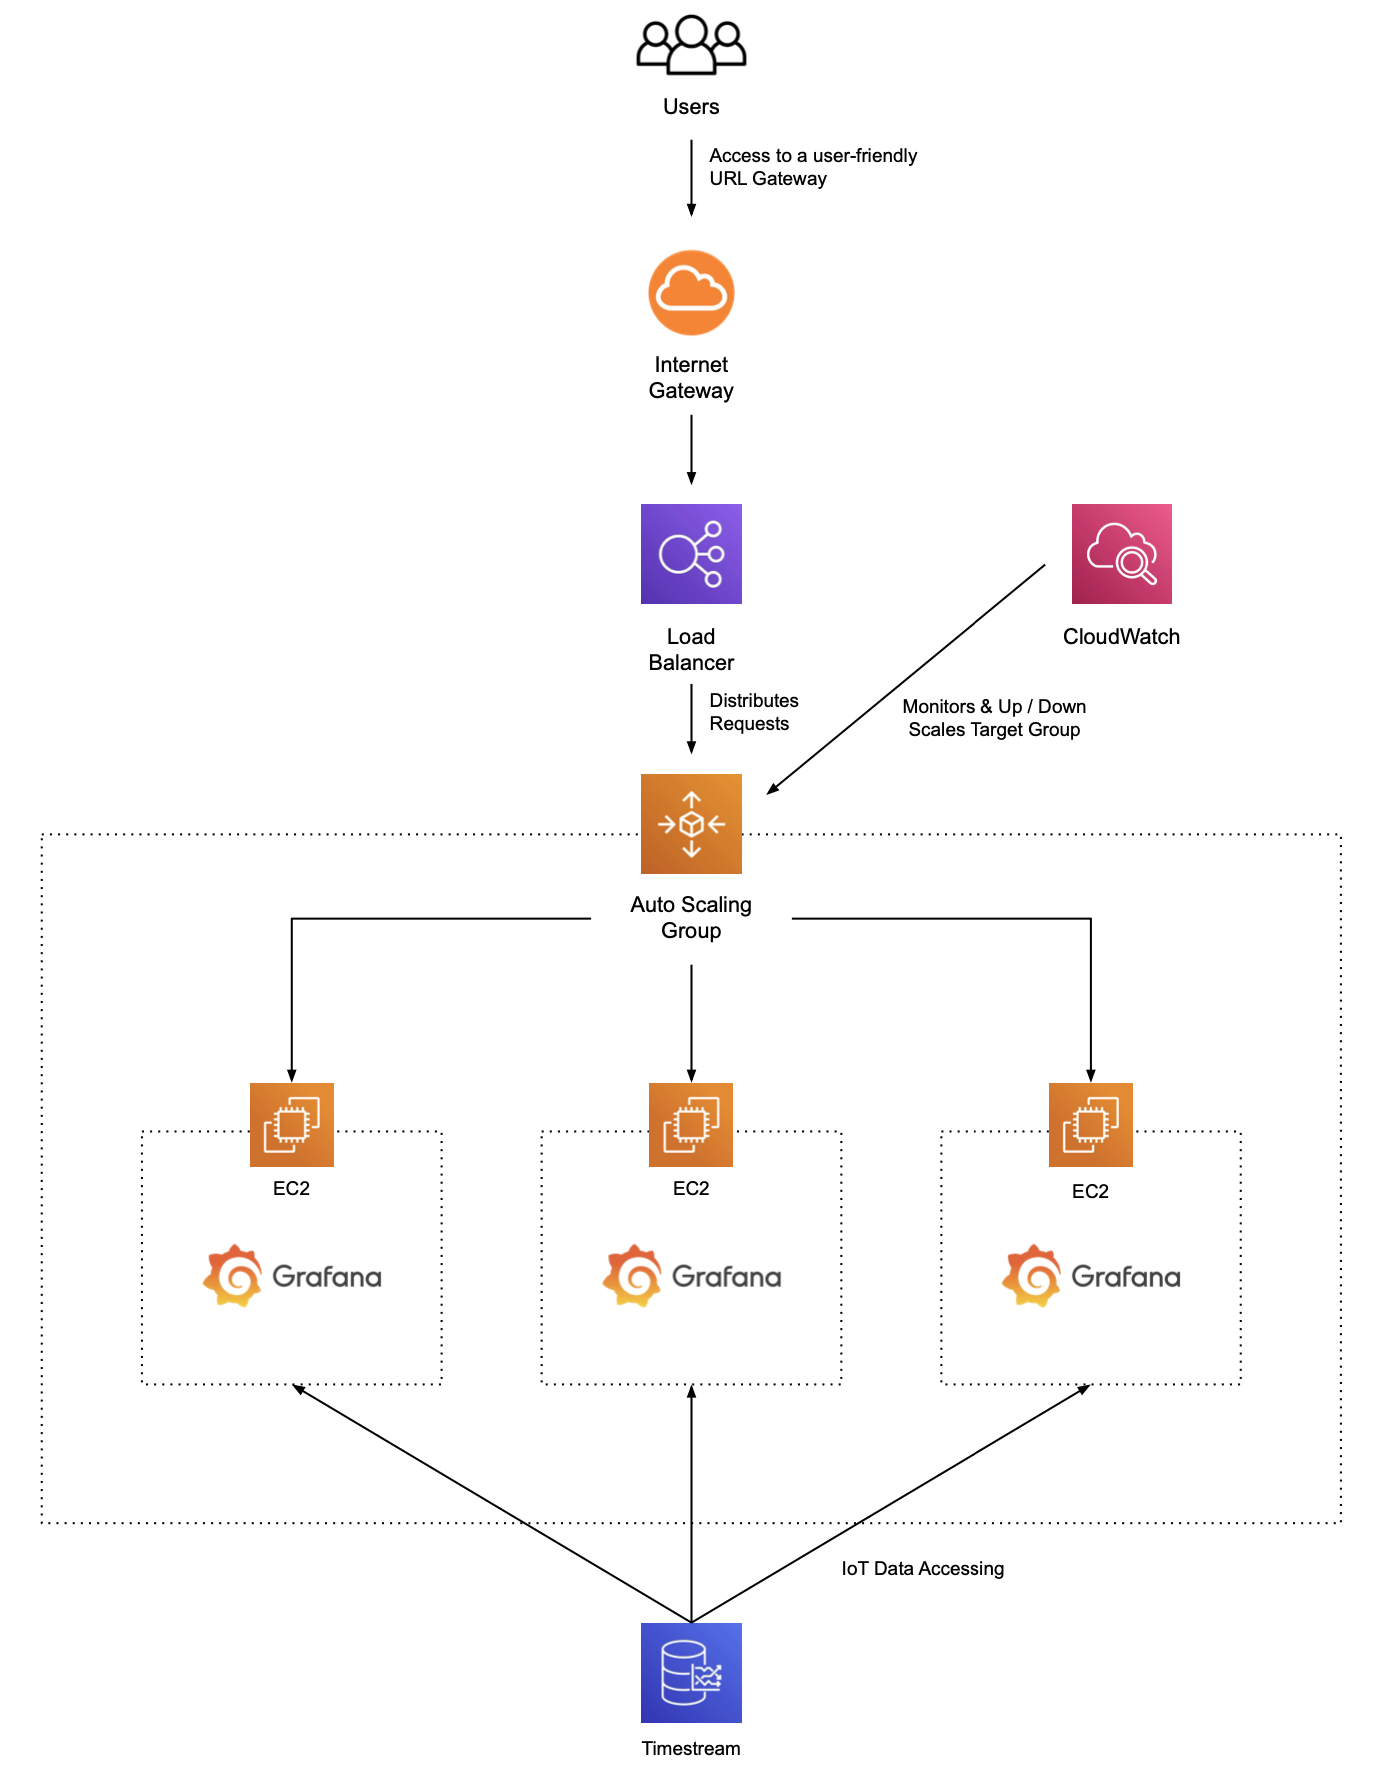
\includegraphics[width=1\linewidth]{images/cloud-computing-clients.png}
    \caption{Data Distributing Pipeline Diagram}
\end{figure}

\subsection{Auto Scaling Group Configuration}

\begin{figure}[H]
    \centering
    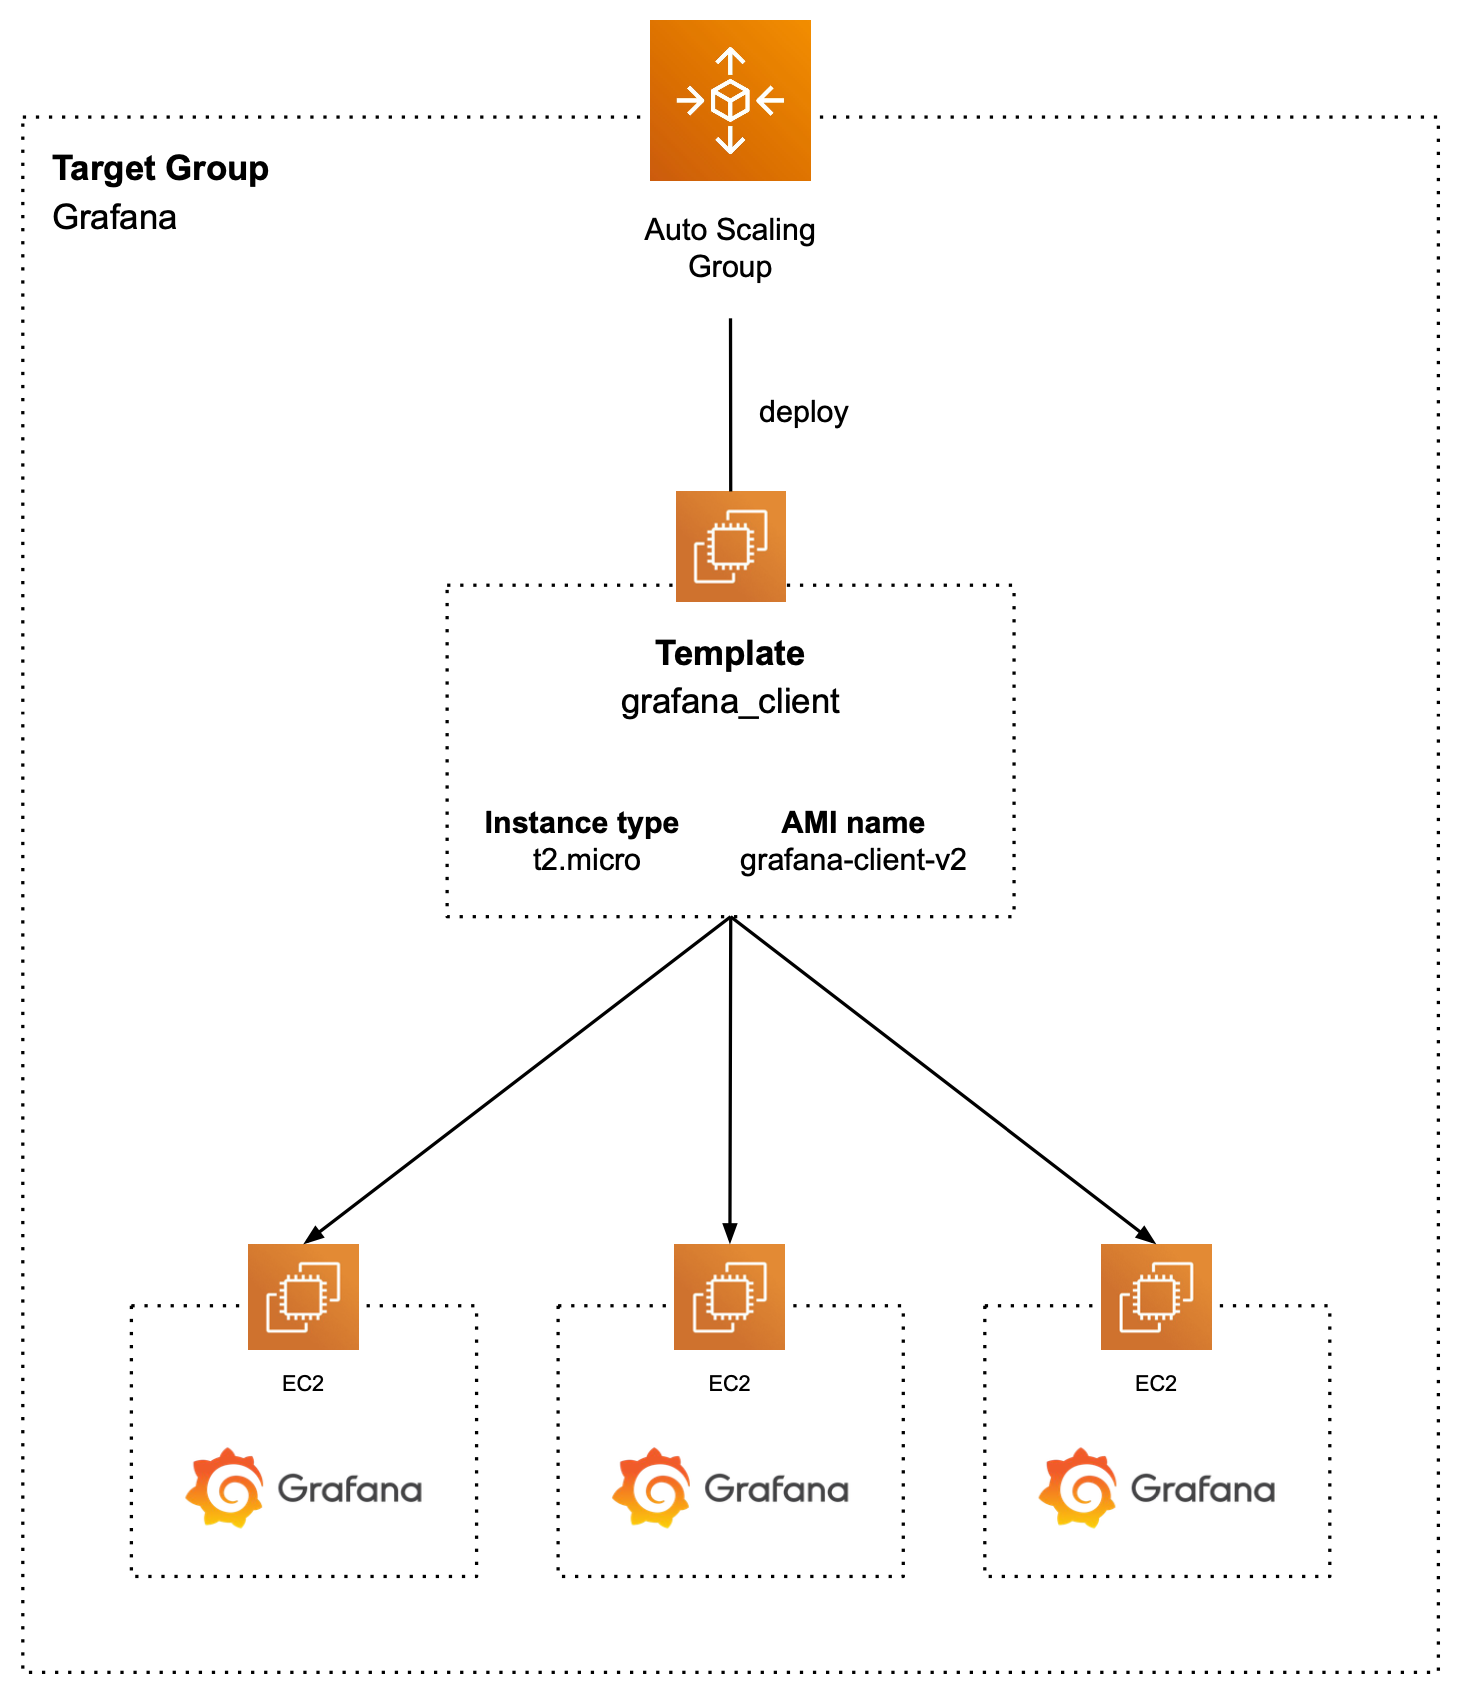
\includegraphics[width=1\linewidth]{images/grafana.png}
    \caption{Auto Scaling Group Pipeline Diagram}
\end{figure}

\newpage
\subsubsection{AMI Configuration}

An Amazon Machine Image (AMI) is a template that contains the software
configuration (operating system, application server, and applications) required
to launch an EC2 instance. A custom AMI using the Amazon Linux 2 operating
system was created to host the Grafana server.

\begin{figure}[H]
    \centering
    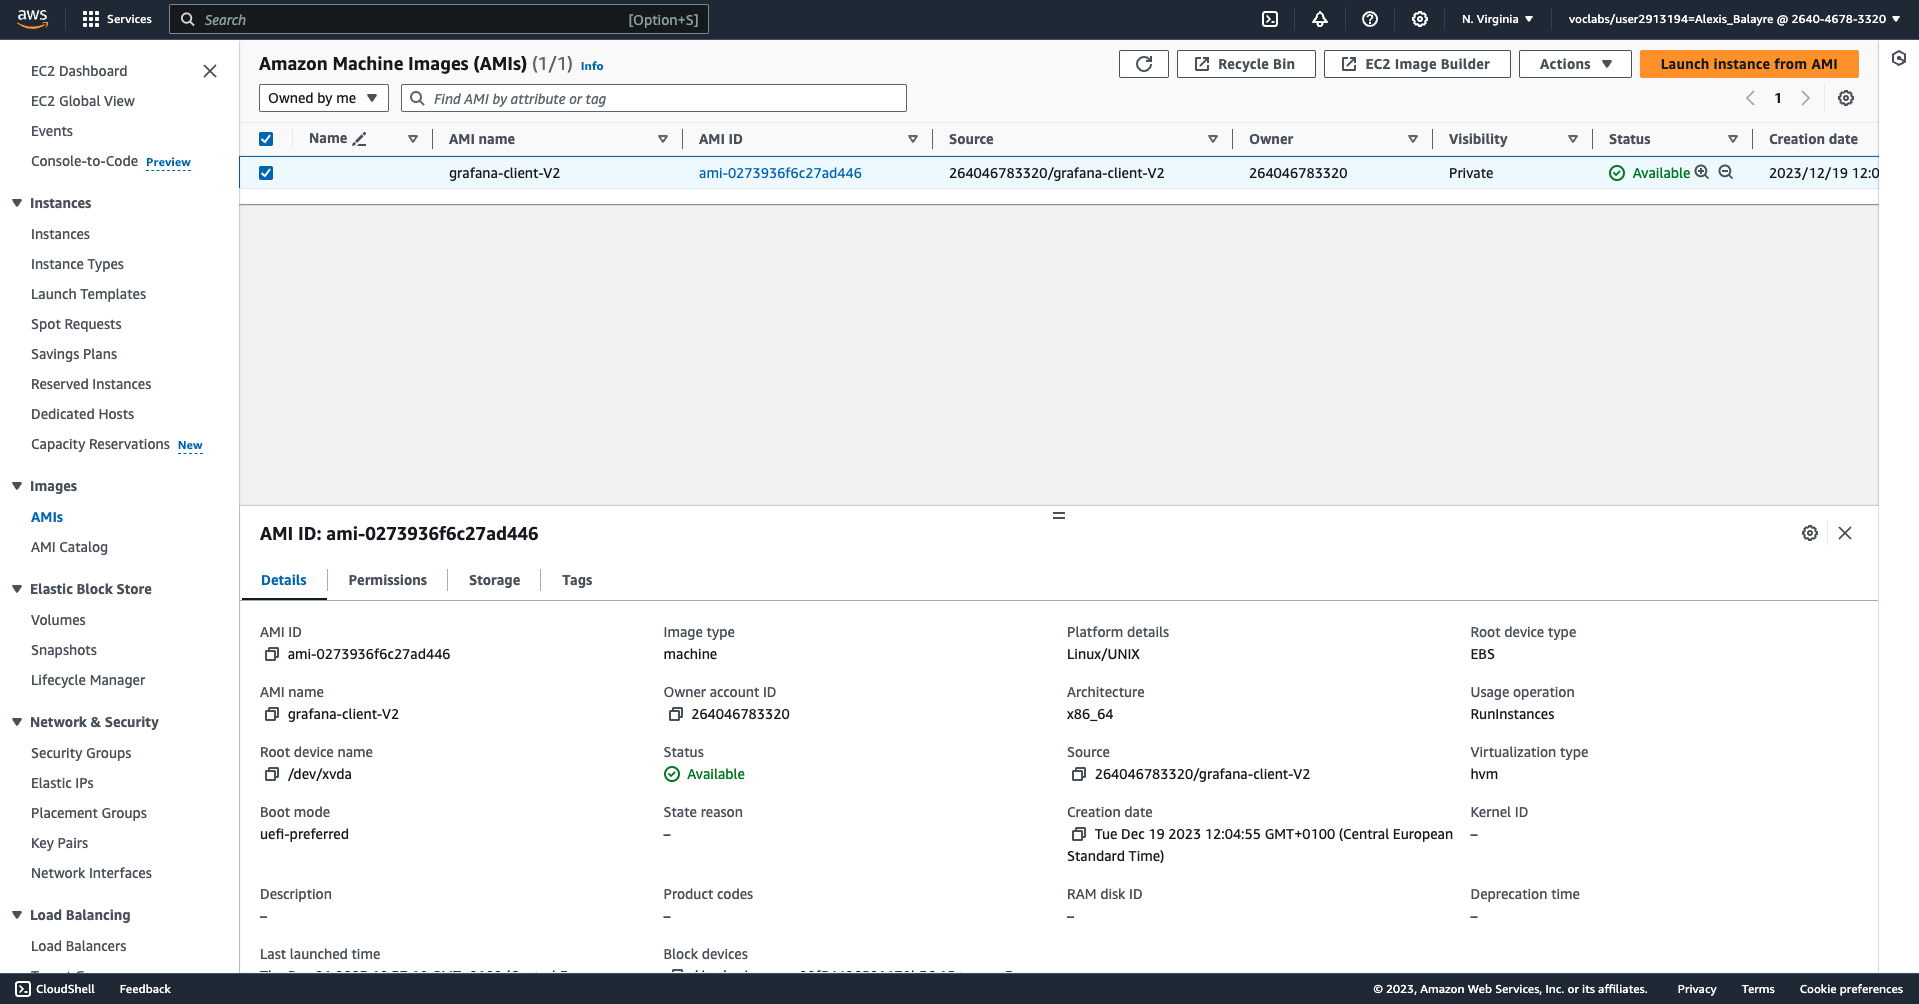
\includegraphics[width=1\linewidth]{images/ami.png}
    \caption{AMI Settings Screenshot}
\end{figure}

\newpage
\subsubsection{Launch Template Configuration}
A launch template was defined to deploy the EC2 instances in the Auto Scaling
Group using the custom AMI. The launch template also defines the instance type,
security group, key pair, and user data.
\begin{figure}[H]
    \centering
    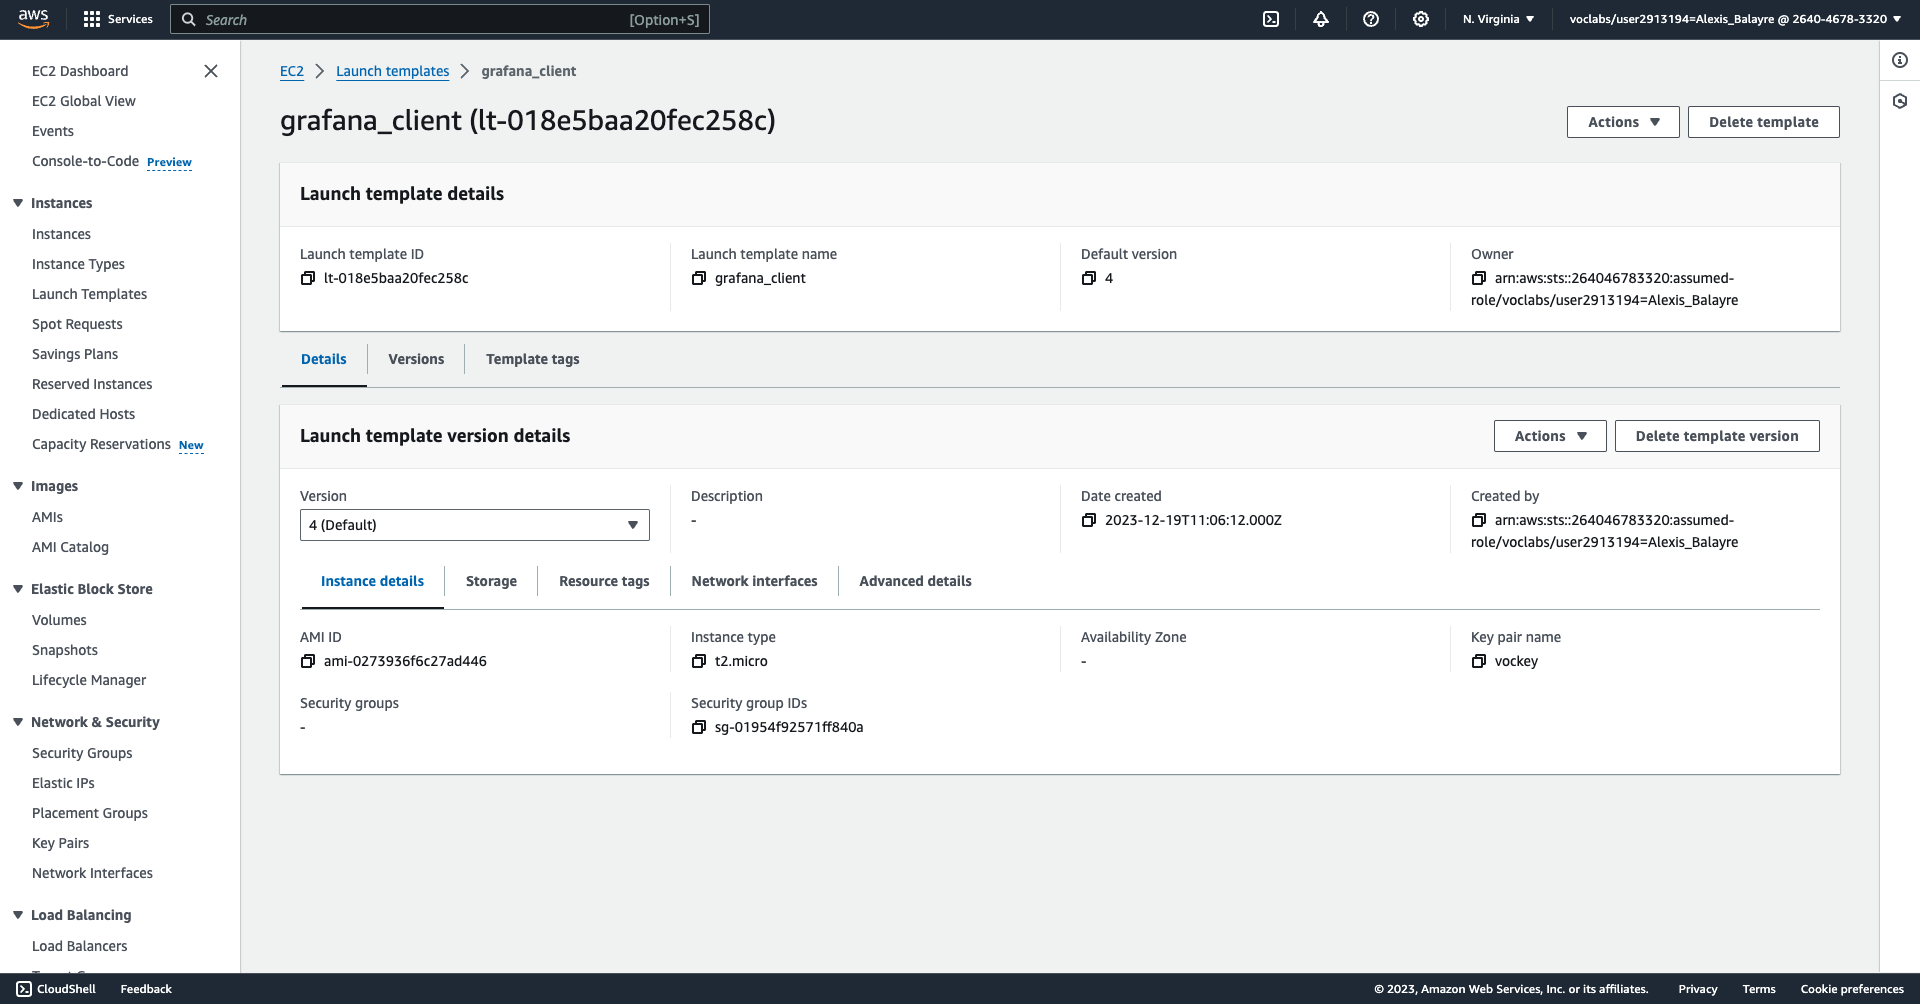
\includegraphics[width=1\linewidth]{images/launch-template.png}
    \caption{Launch Template Settings Screenshot}
\end{figure}

\newpage
\subsubsection{Auto Scaling Group Configuration}
An Auto Scaling Group was created to manage the EC2 instances of the
Distributing Data Pipeline. The Auto Scaling Group is configured to use the
launch template and to scale between 1 and 5 instances, depending on the CPU
utilization of the instances. The Auto Scaling Group also defines the target
group and load balancer to use for distributing traffic between the instances.
\begin{figure}[H]
    \centering
    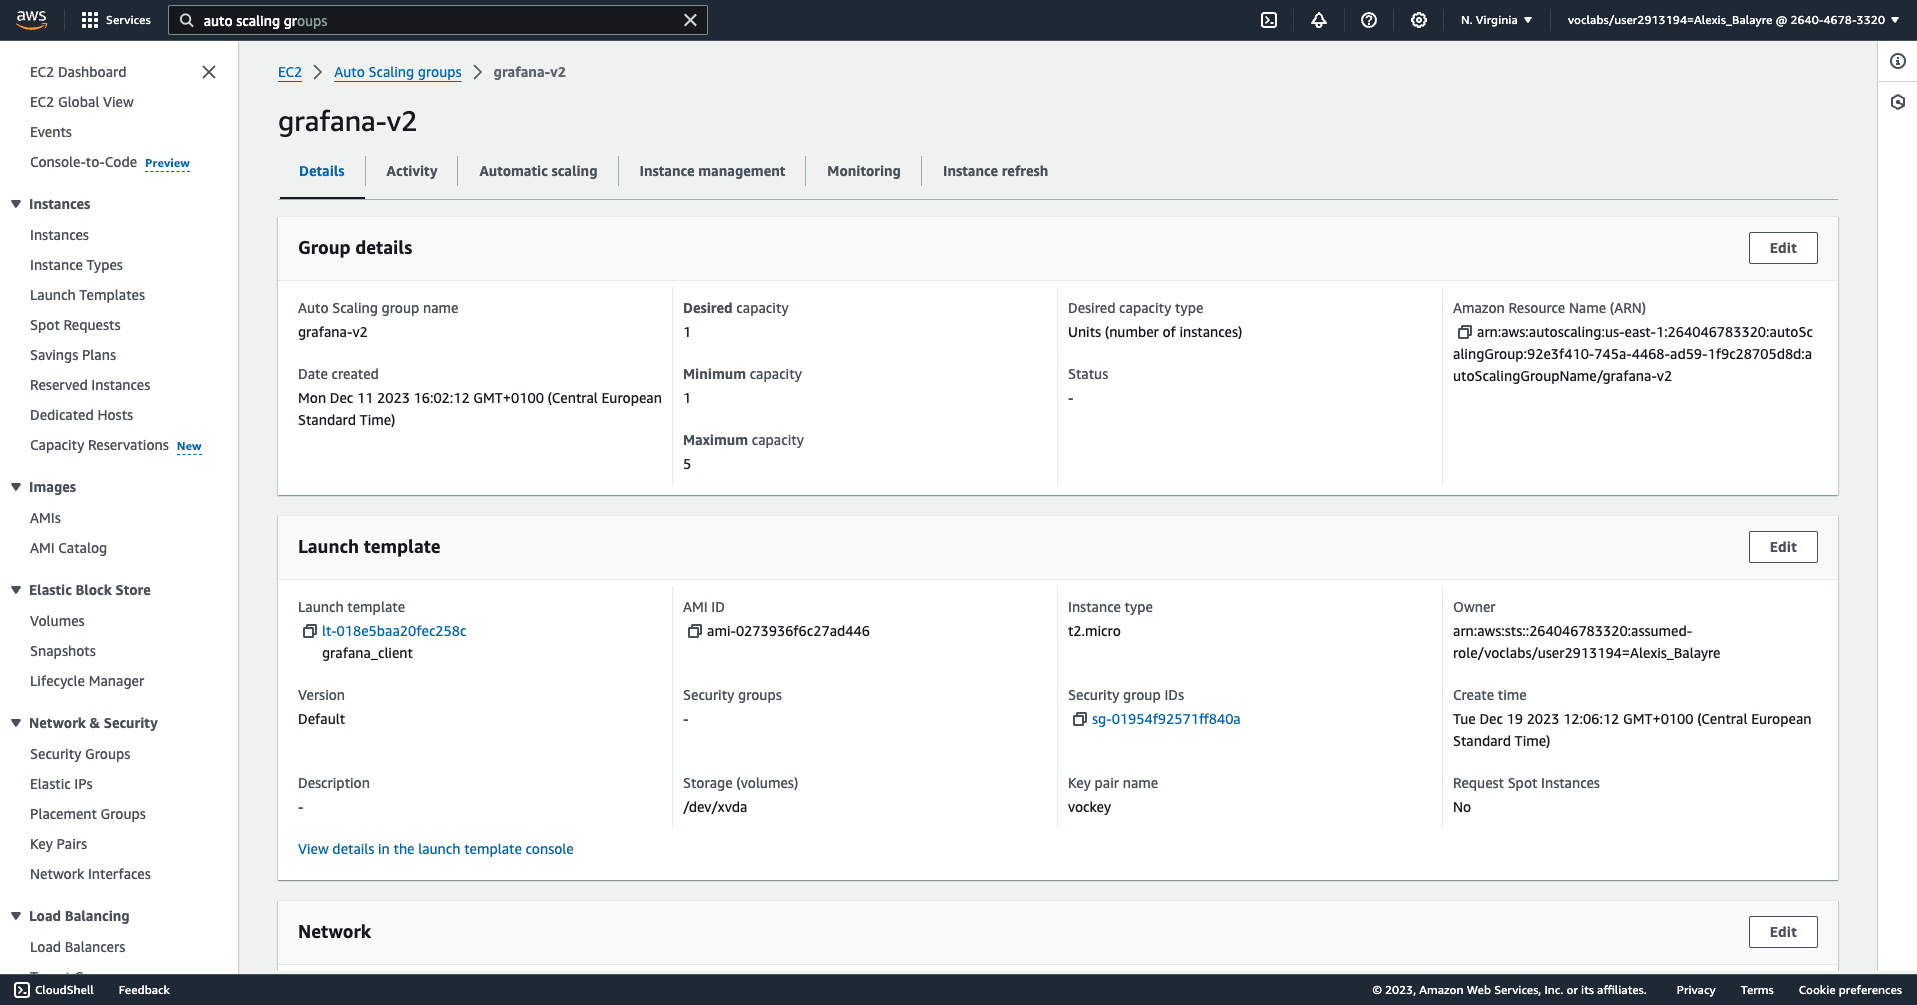
\includegraphics[width=1\linewidth]{images/auto-scaling-group.png}
    \caption{Auto Scaling Group Settings Screenshot}
\end{figure}

The Auto Scaling Group is configured to use the following scaling policy:
\begin{itemize}
    \item \textbf{Scale-out Policy:} The scale-out policy is triggered when the average CPU utilization of the instances is greater than 60\% for 3 minutes. The scale-out policy adds 1 instance to the Auto Scaling Group.
    \item \textbf{Scale-in Policy:} The scale-in policy is triggered when the average CPU utilization of the instances is less than 42\% for 15 minutes. The scale-in policy removes 1 instance from the Auto Scaling Group.
    \item \textbf{Cooldown Period:} The cooldown period is set to 60 seconds to prevent the Auto Scaling Group from scaling in or out too quickly.
\end{itemize}

\begin{figure}[H]
    \centering
    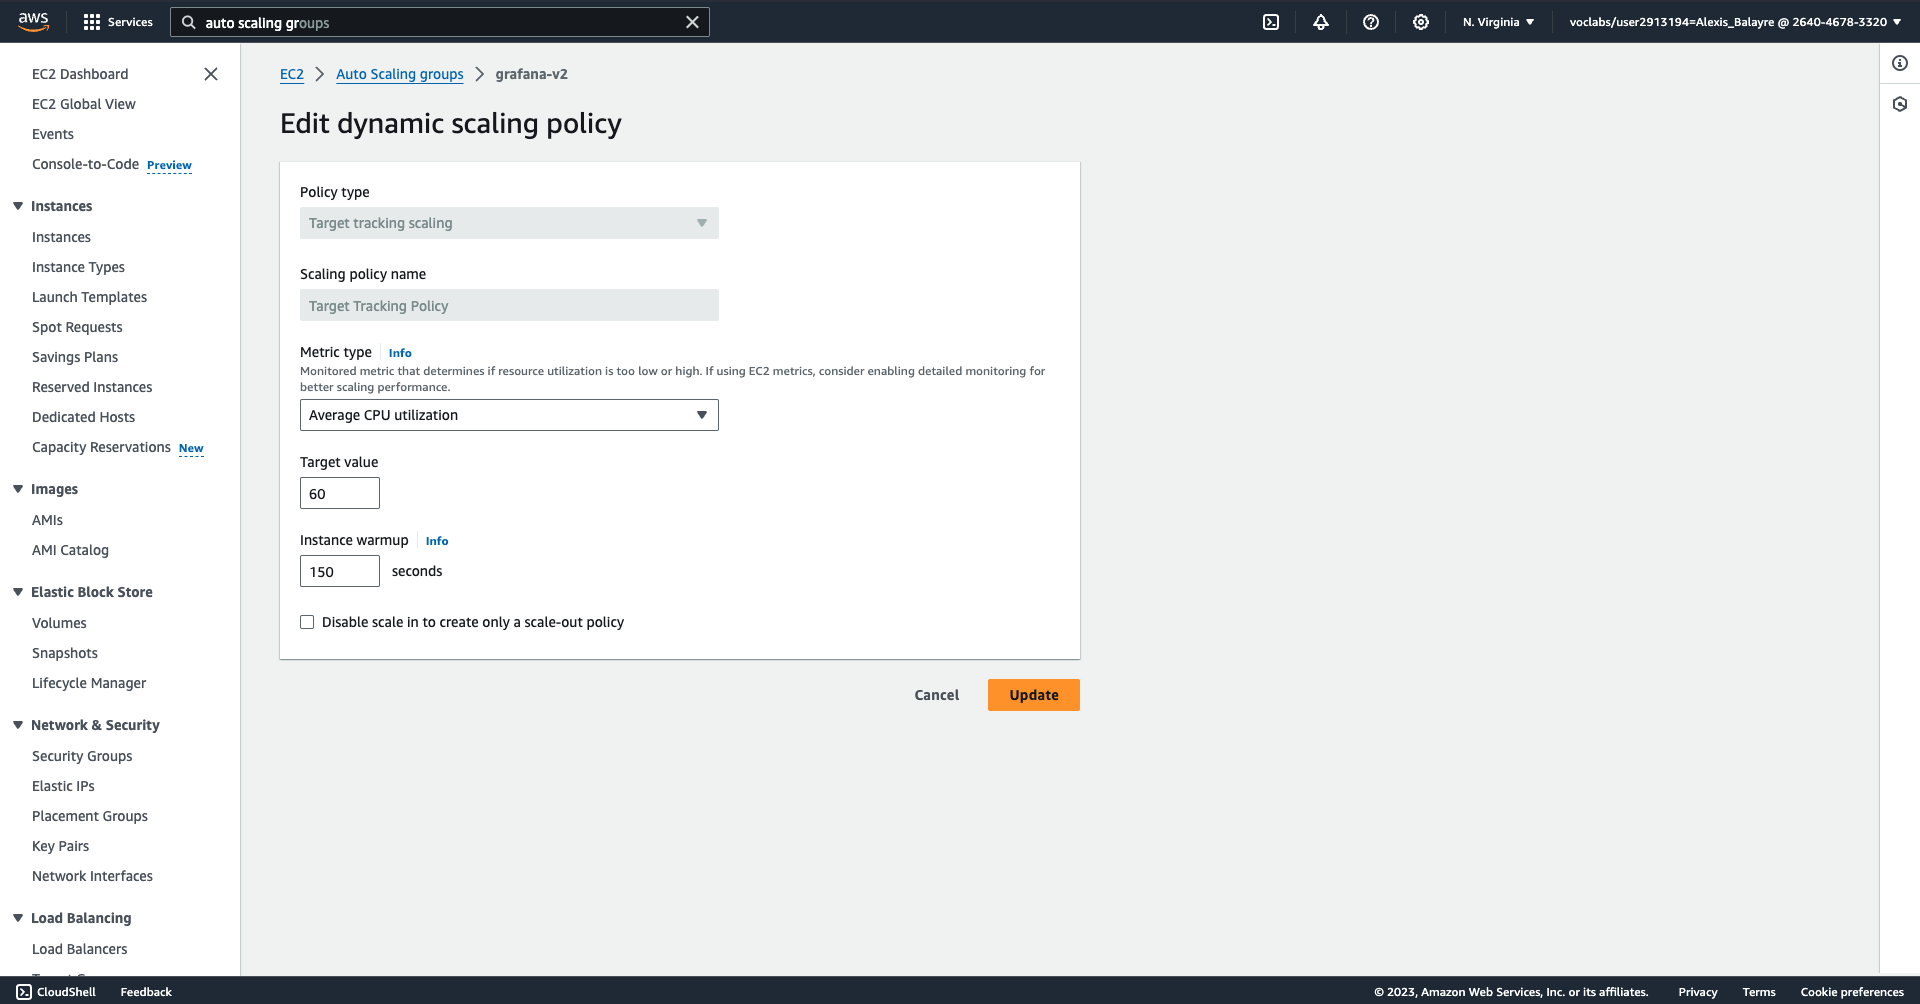
\includegraphics[width=1\linewidth]{images/scaling-policy.png}
    \caption{Scaling Policy Settings Screenshot}
\end{figure}

\subsubsection{Target Group Configuration}

A target group was created to distribute traffic between the EC2 instances of
the Auto Scaling Group.

\begin{figure}[H]
    \centering
    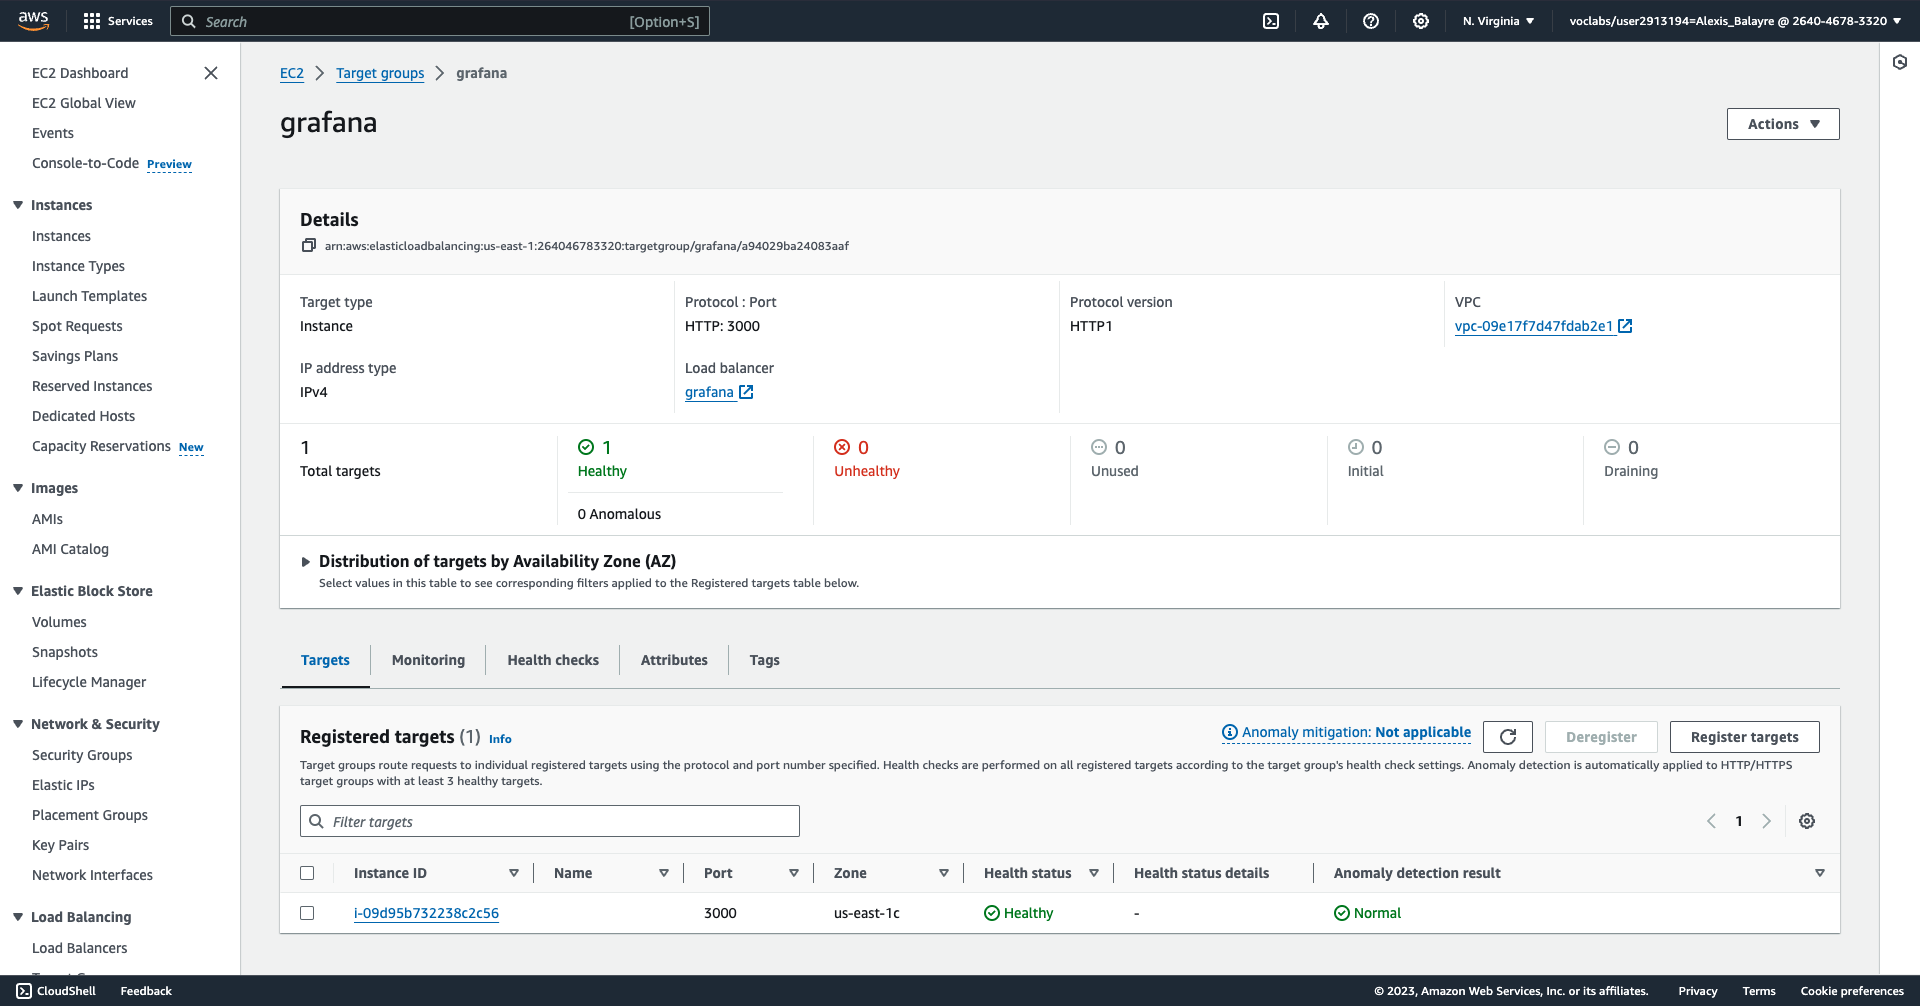
\includegraphics[width=1\linewidth]{images/target-group.png}
    \caption{Target Group Settings Screenshot}
\end{figure}

\newpage
\subsubsection{Load Balancer Configuration}
A load balancer was created to distribute traffic between the EC2 instances of
the Auto Scaling Group. The load balancer is configured to use the target group
and to listen on port 80.

\begin{figure}[H]
    \centering
    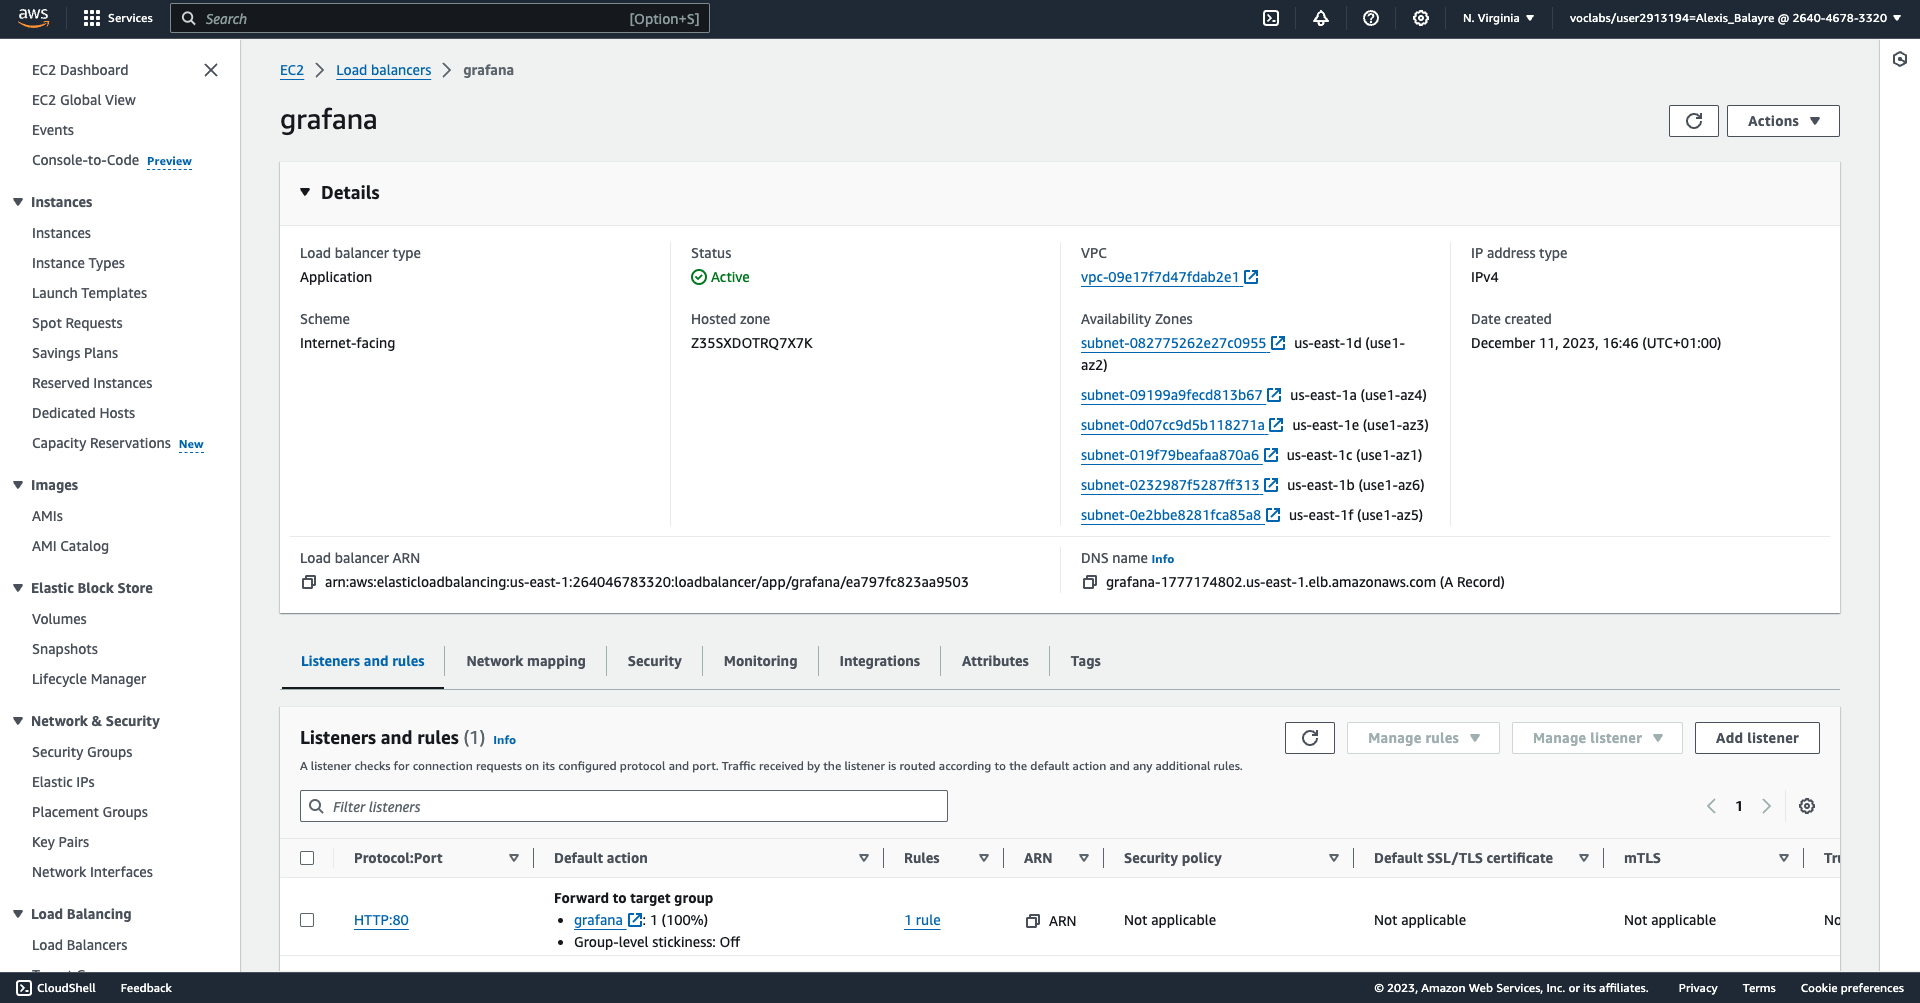
\includegraphics[width=1\linewidth]{images/load-balancer.png}
    \caption{Load Balancer Settings Screenshot}
\end{figure}

\newpage
\section{Pipeline of the Project}

\begin{figure}[H]
    \centering
    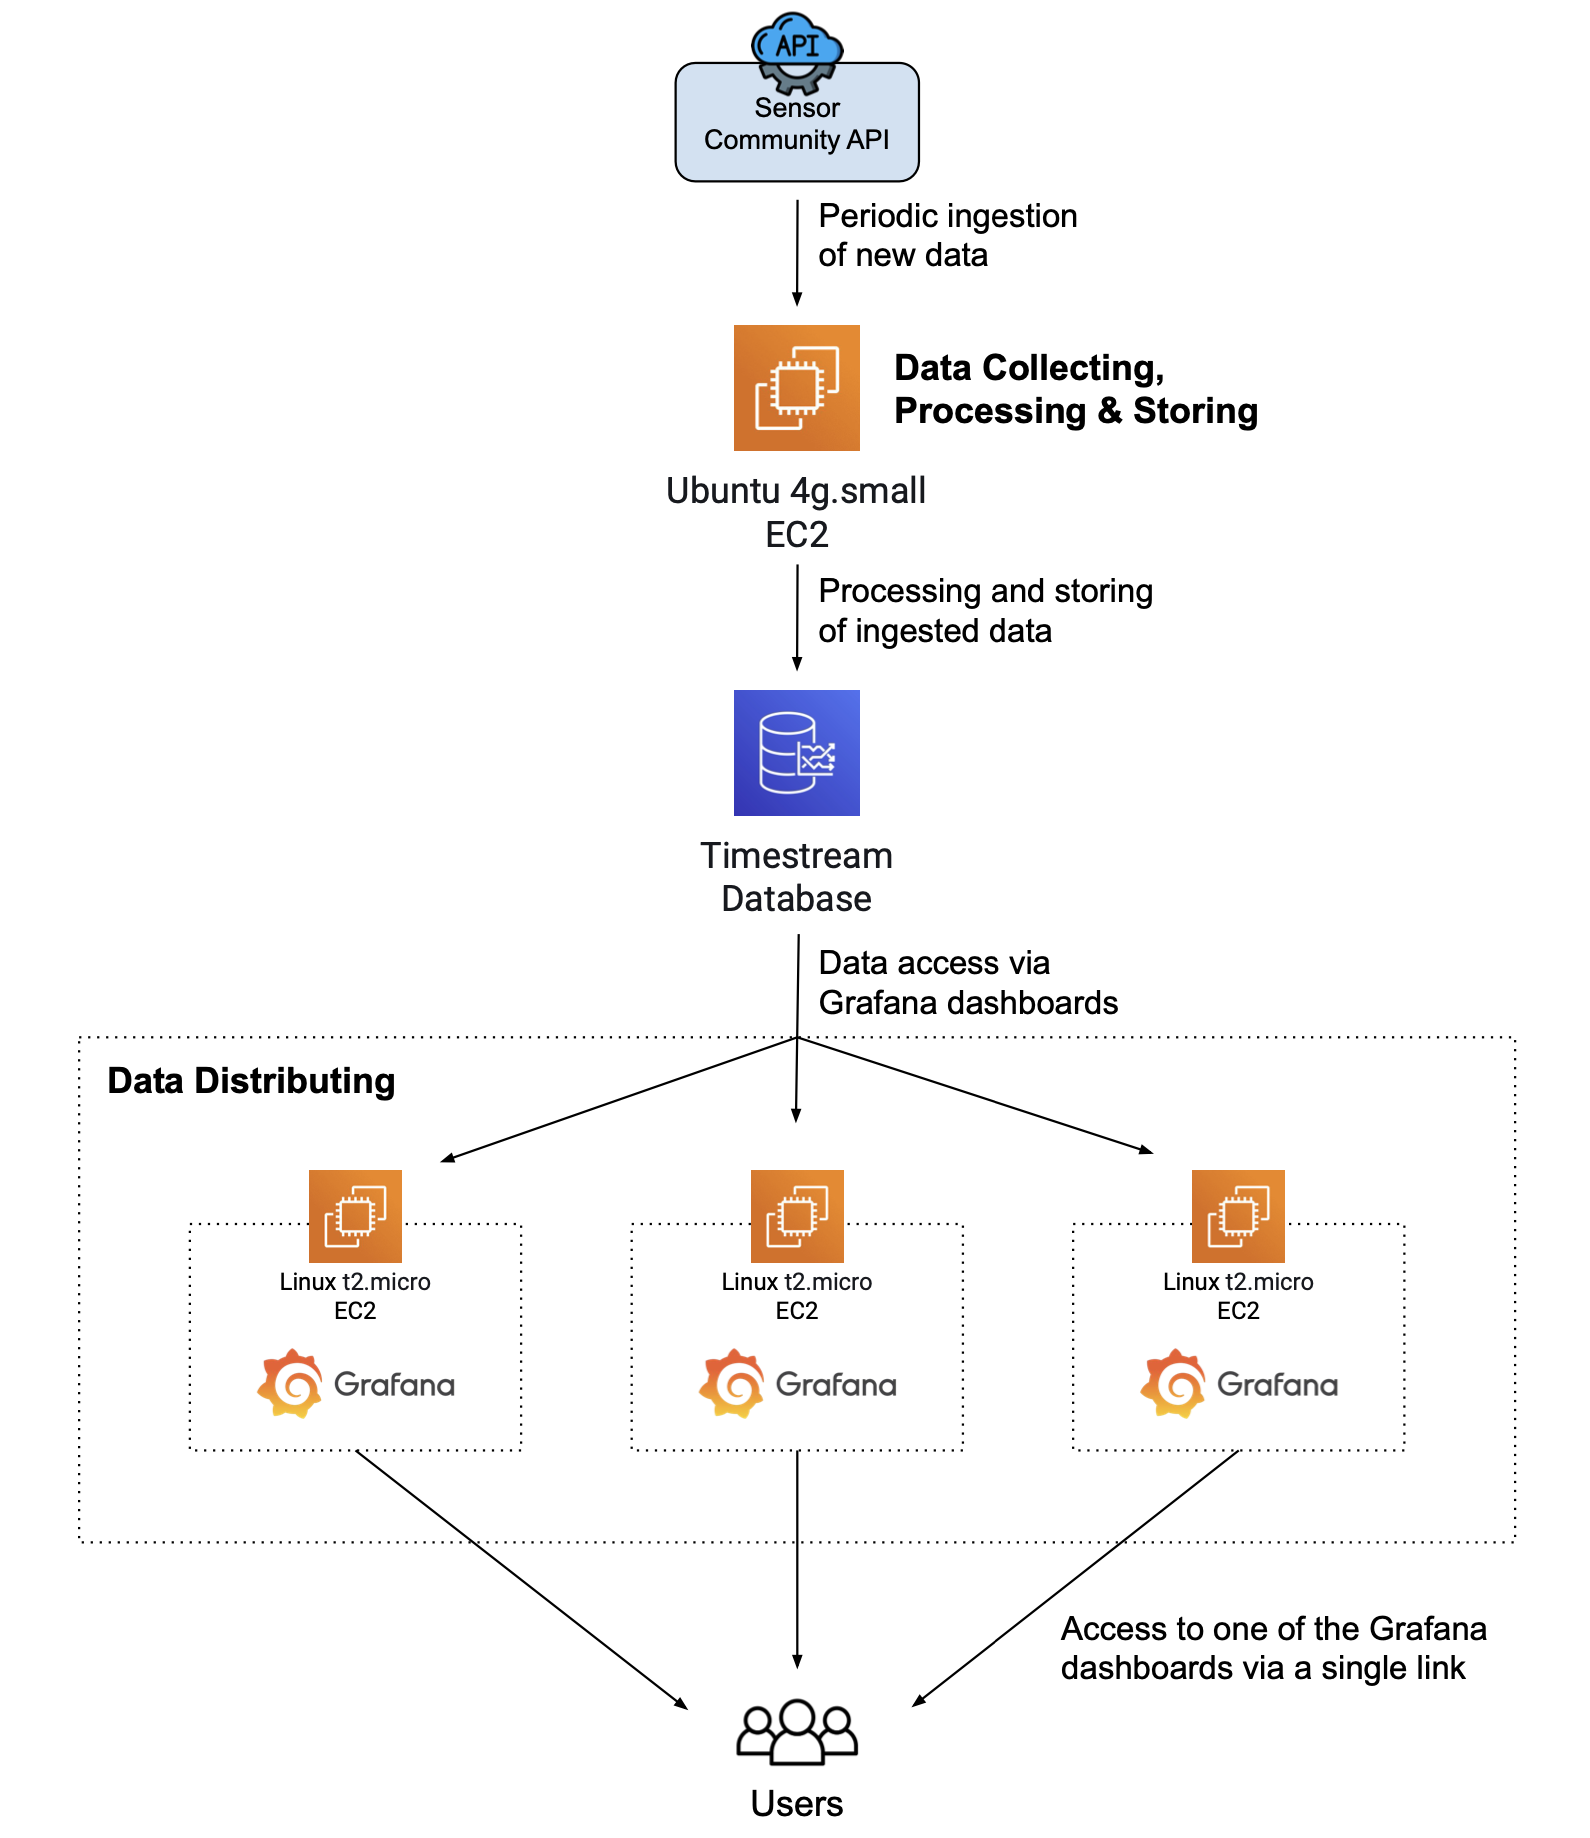
\includegraphics[width=1\linewidth]{images/pipeline.png}
    \caption{Data Distributing Pipeline Diagram}
\end{figure}

\newpage
\chapter{Results \& Discussion}

\section{Results}
\subsection{Accessing the Data - Grafana Dashboard}

The Grafana dashboard, a vital tool in air quality monitoring, is accessible at
the following URL:
\href{http://grafana-1777174802.us-east-1.elb.amazonaws.com/d/f8742187-f440-4ee8-96cc-bad5af8edef1/air-quality-monitoring}{Air
    Quality Monitoring Dashboard}.

The Grafana dashboard provides an interactive interface enabling users to
analyse air quality data. Users can customise the time interval, measurement
value and location ID. The dashboard consists of five main panels, each
providing unique information::
\begin{enumerate}
    \item \textbf{Measure Value Evolution:} This panel shows the evolution of the selected measure value in the selected location over the selected time range.
    \item \textbf{Max AQI:} This panel shows the maximum AQI value in the selected location over the selected time range.
    \item \textbf{Mean AQI:} This panel shows the mean AQI value in the selected location over the selected time range.
    \item \textbf{AQI Map:} This panel shows the AQI value of each location on a map.
    \item \textbf{IoT Data:} This panel shows all the data collected by the IoT sensors related to the selected
\end{enumerate}

\begin{figure}[H]
    \centering
    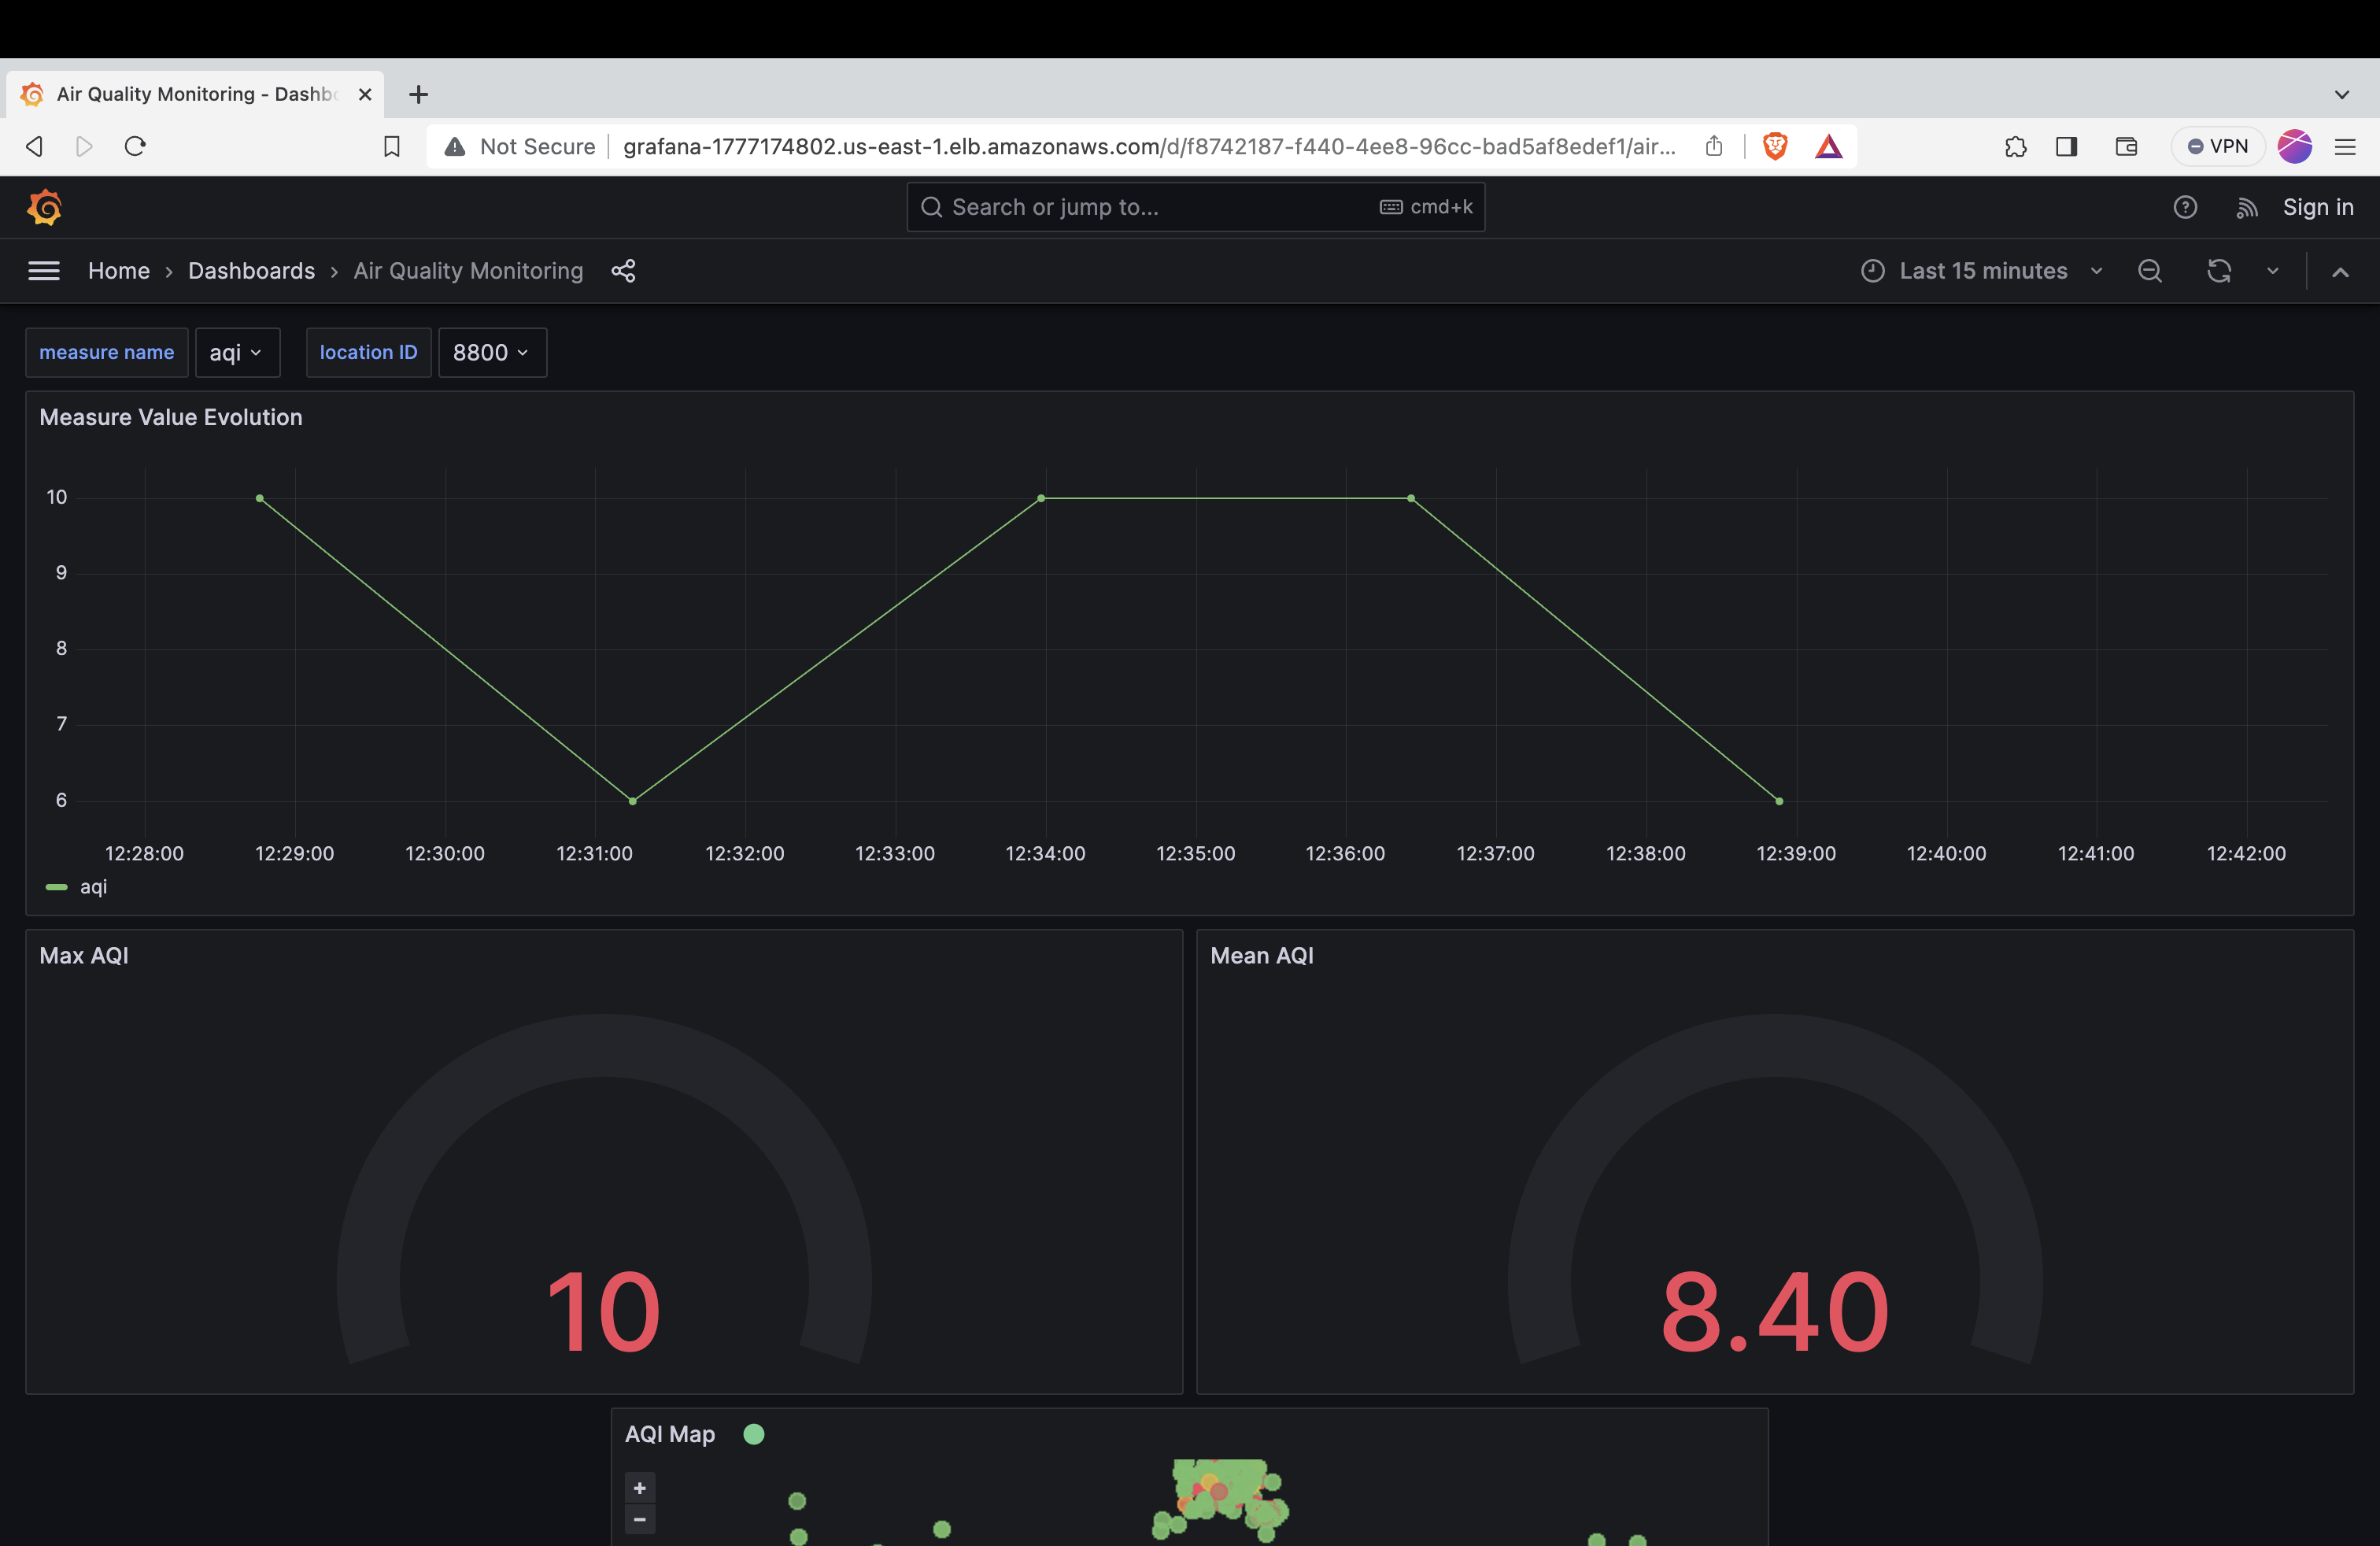
\includegraphics[width=1\linewidth]{images/grafana-1.png}
    \caption{Grafana Dashboard: Measure Value Evolution, Max \& Mean AQI}\label{fig:grafana-main-panel-1}
\end{figure}

\begin{figure}[H]
    \centering
    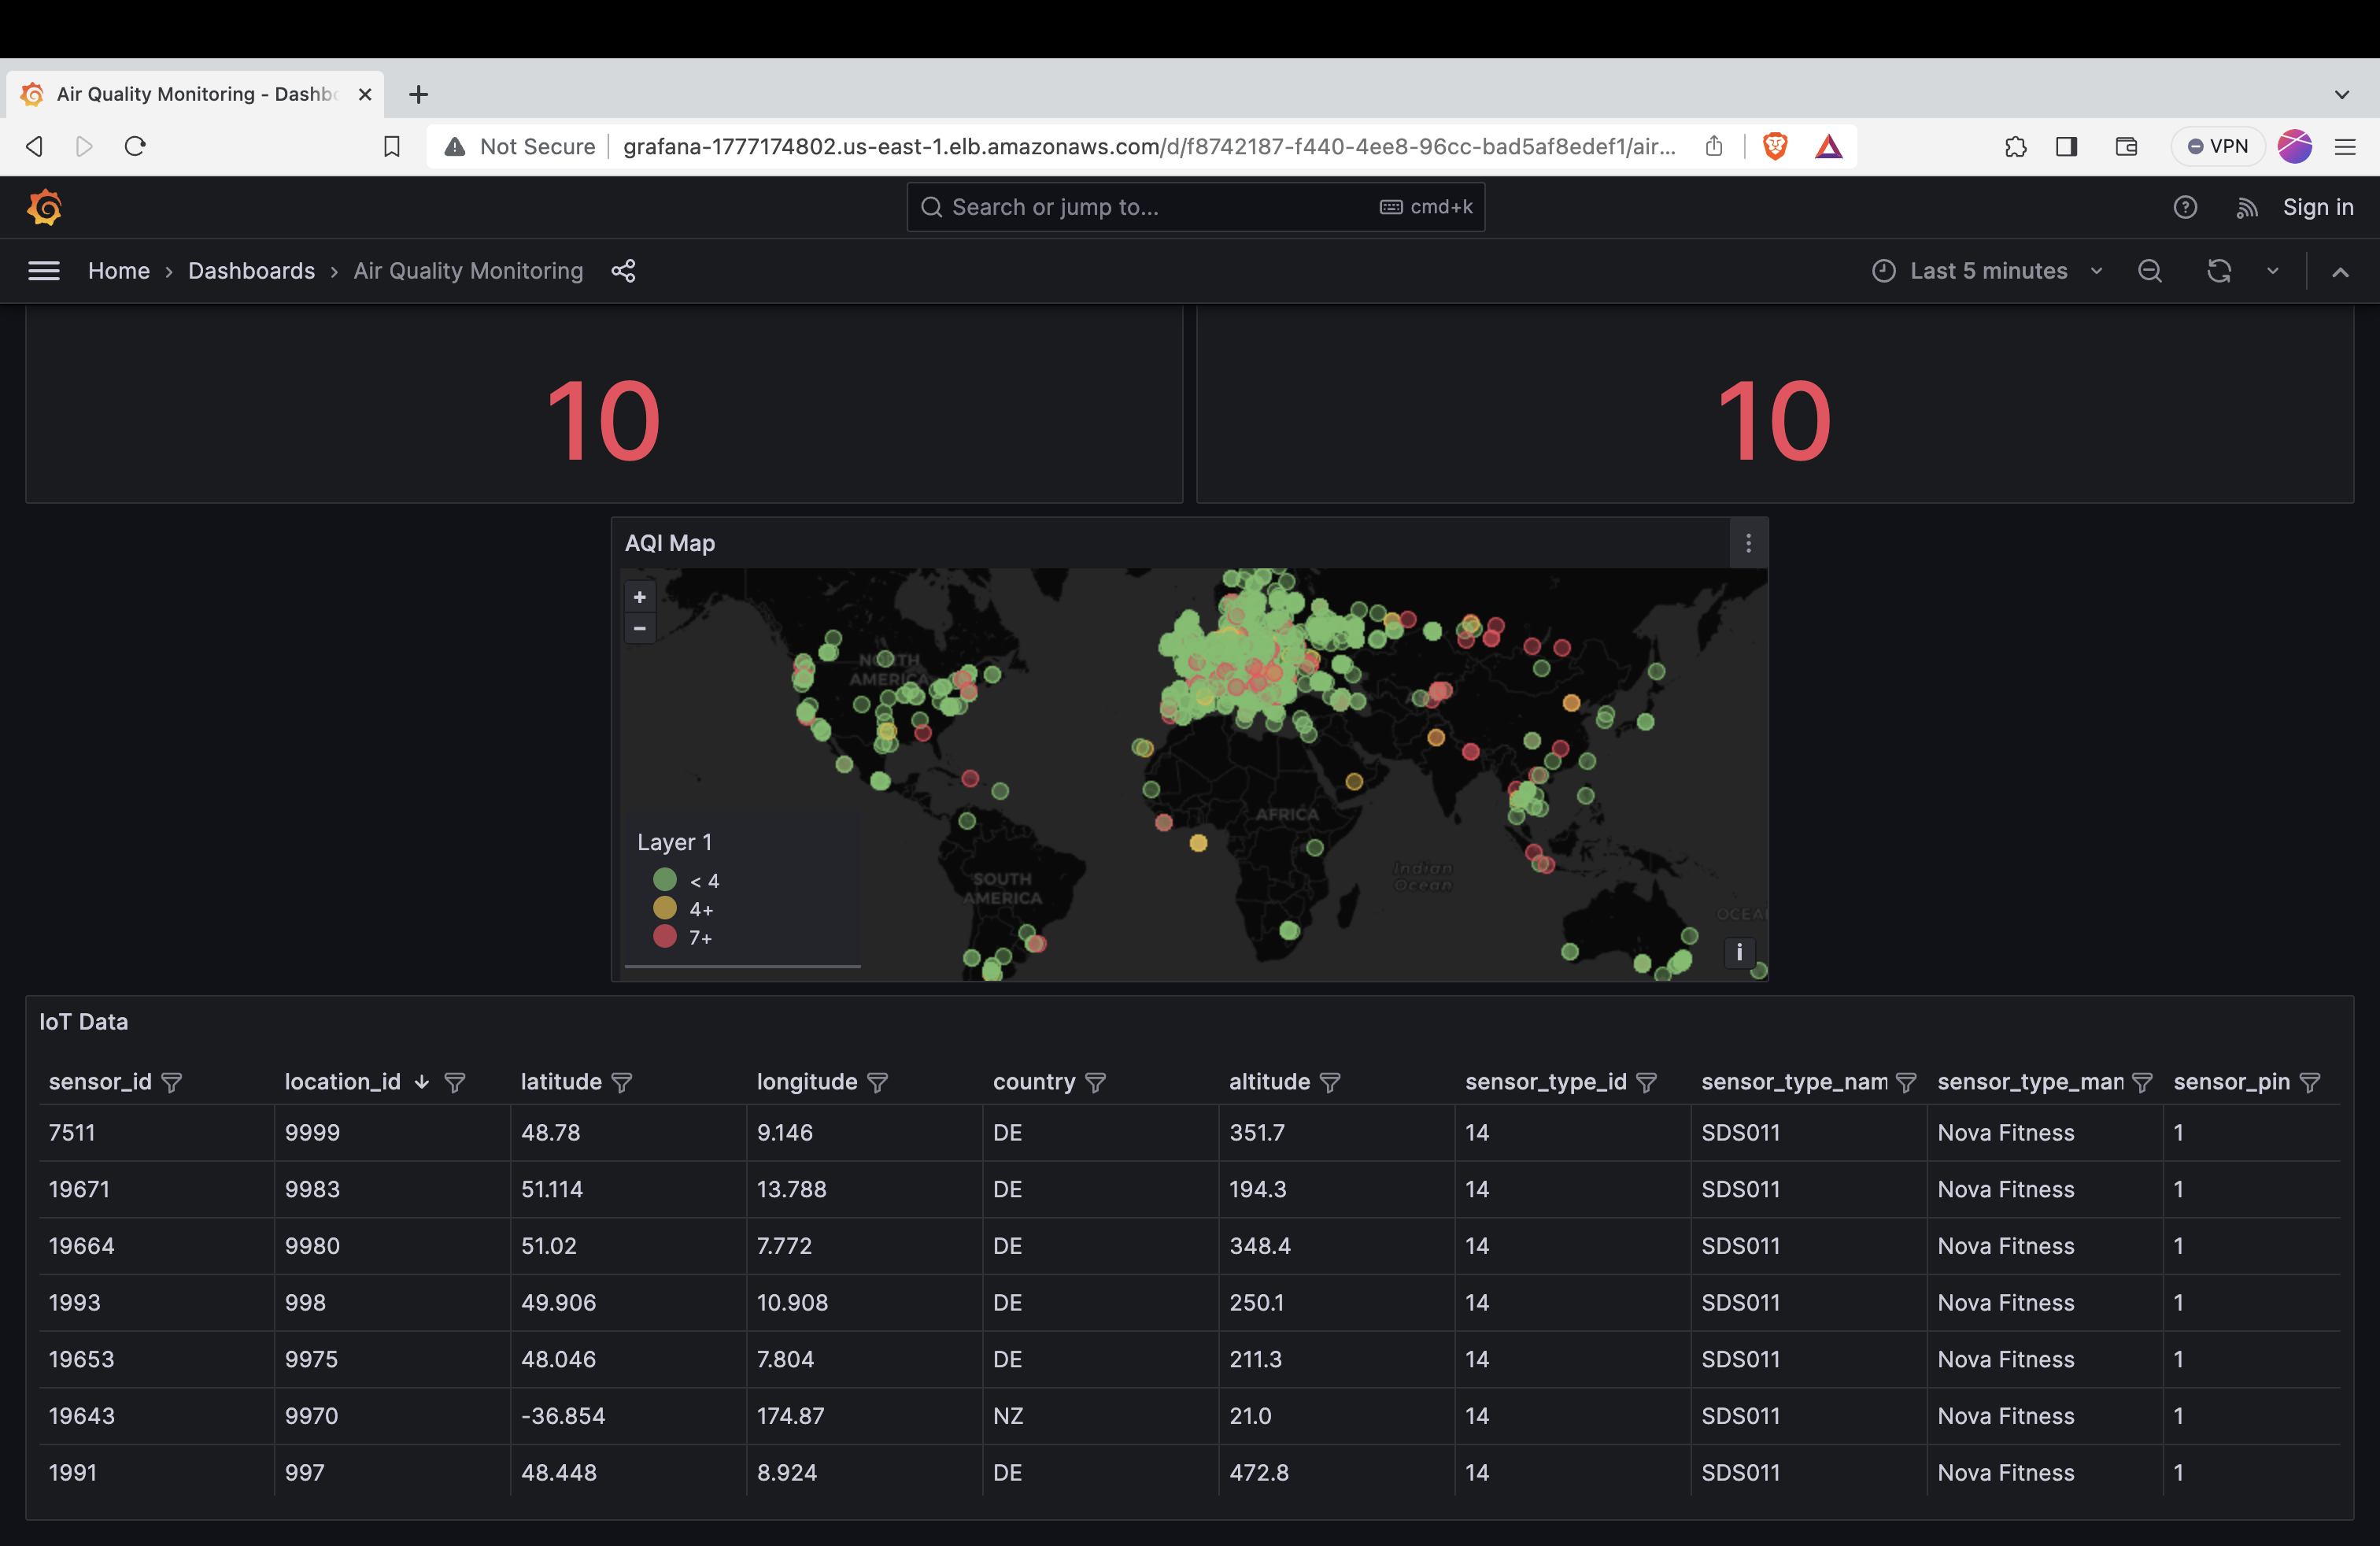
\includegraphics[width=1\linewidth]{images/grafana-2.png}
    \caption{Grafana Dashboard: AQI Map \& IoT Data}\label{fig:grafana-main-panel-2}
\end{figure}

\begin{figure}[H]
    \centering
    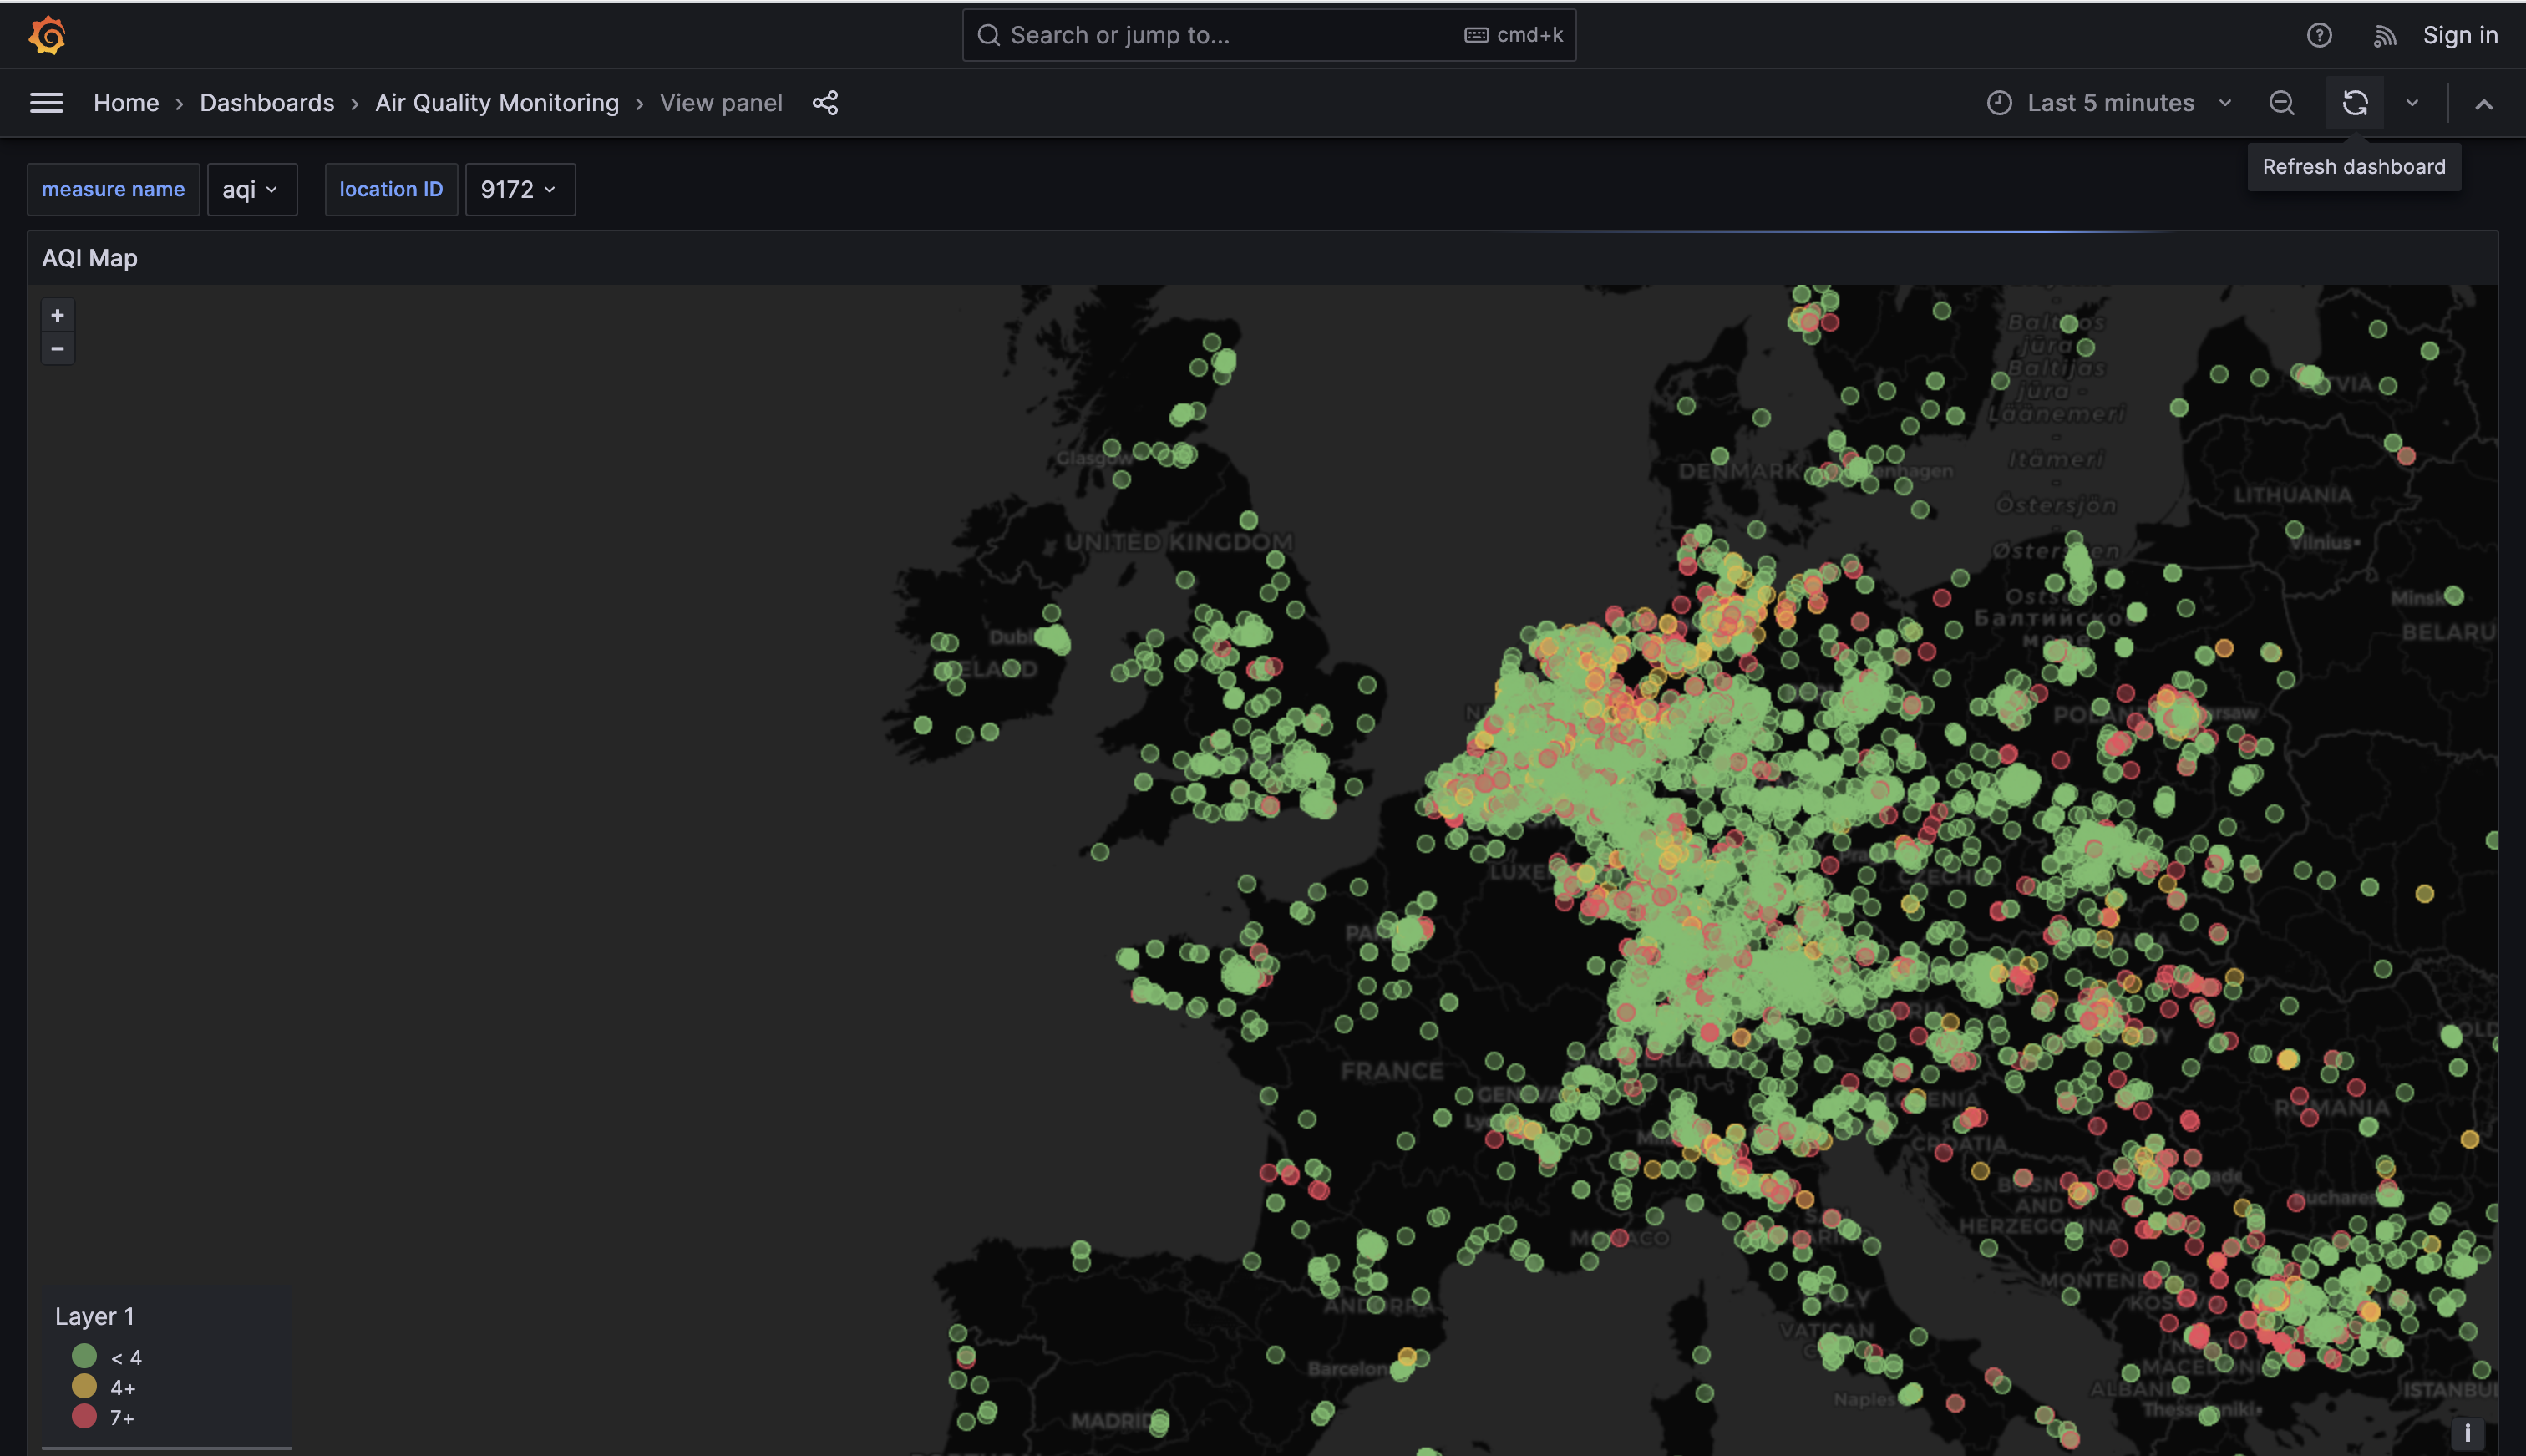
\includegraphics[width=1\linewidth]{images/grafana-4.png}
    \caption{Grafana Dashboard AQI Map Panel}\label{fig:grafana-aqi-map-panel}
\end{figure}

\begin{figure}[H]
    \centering
    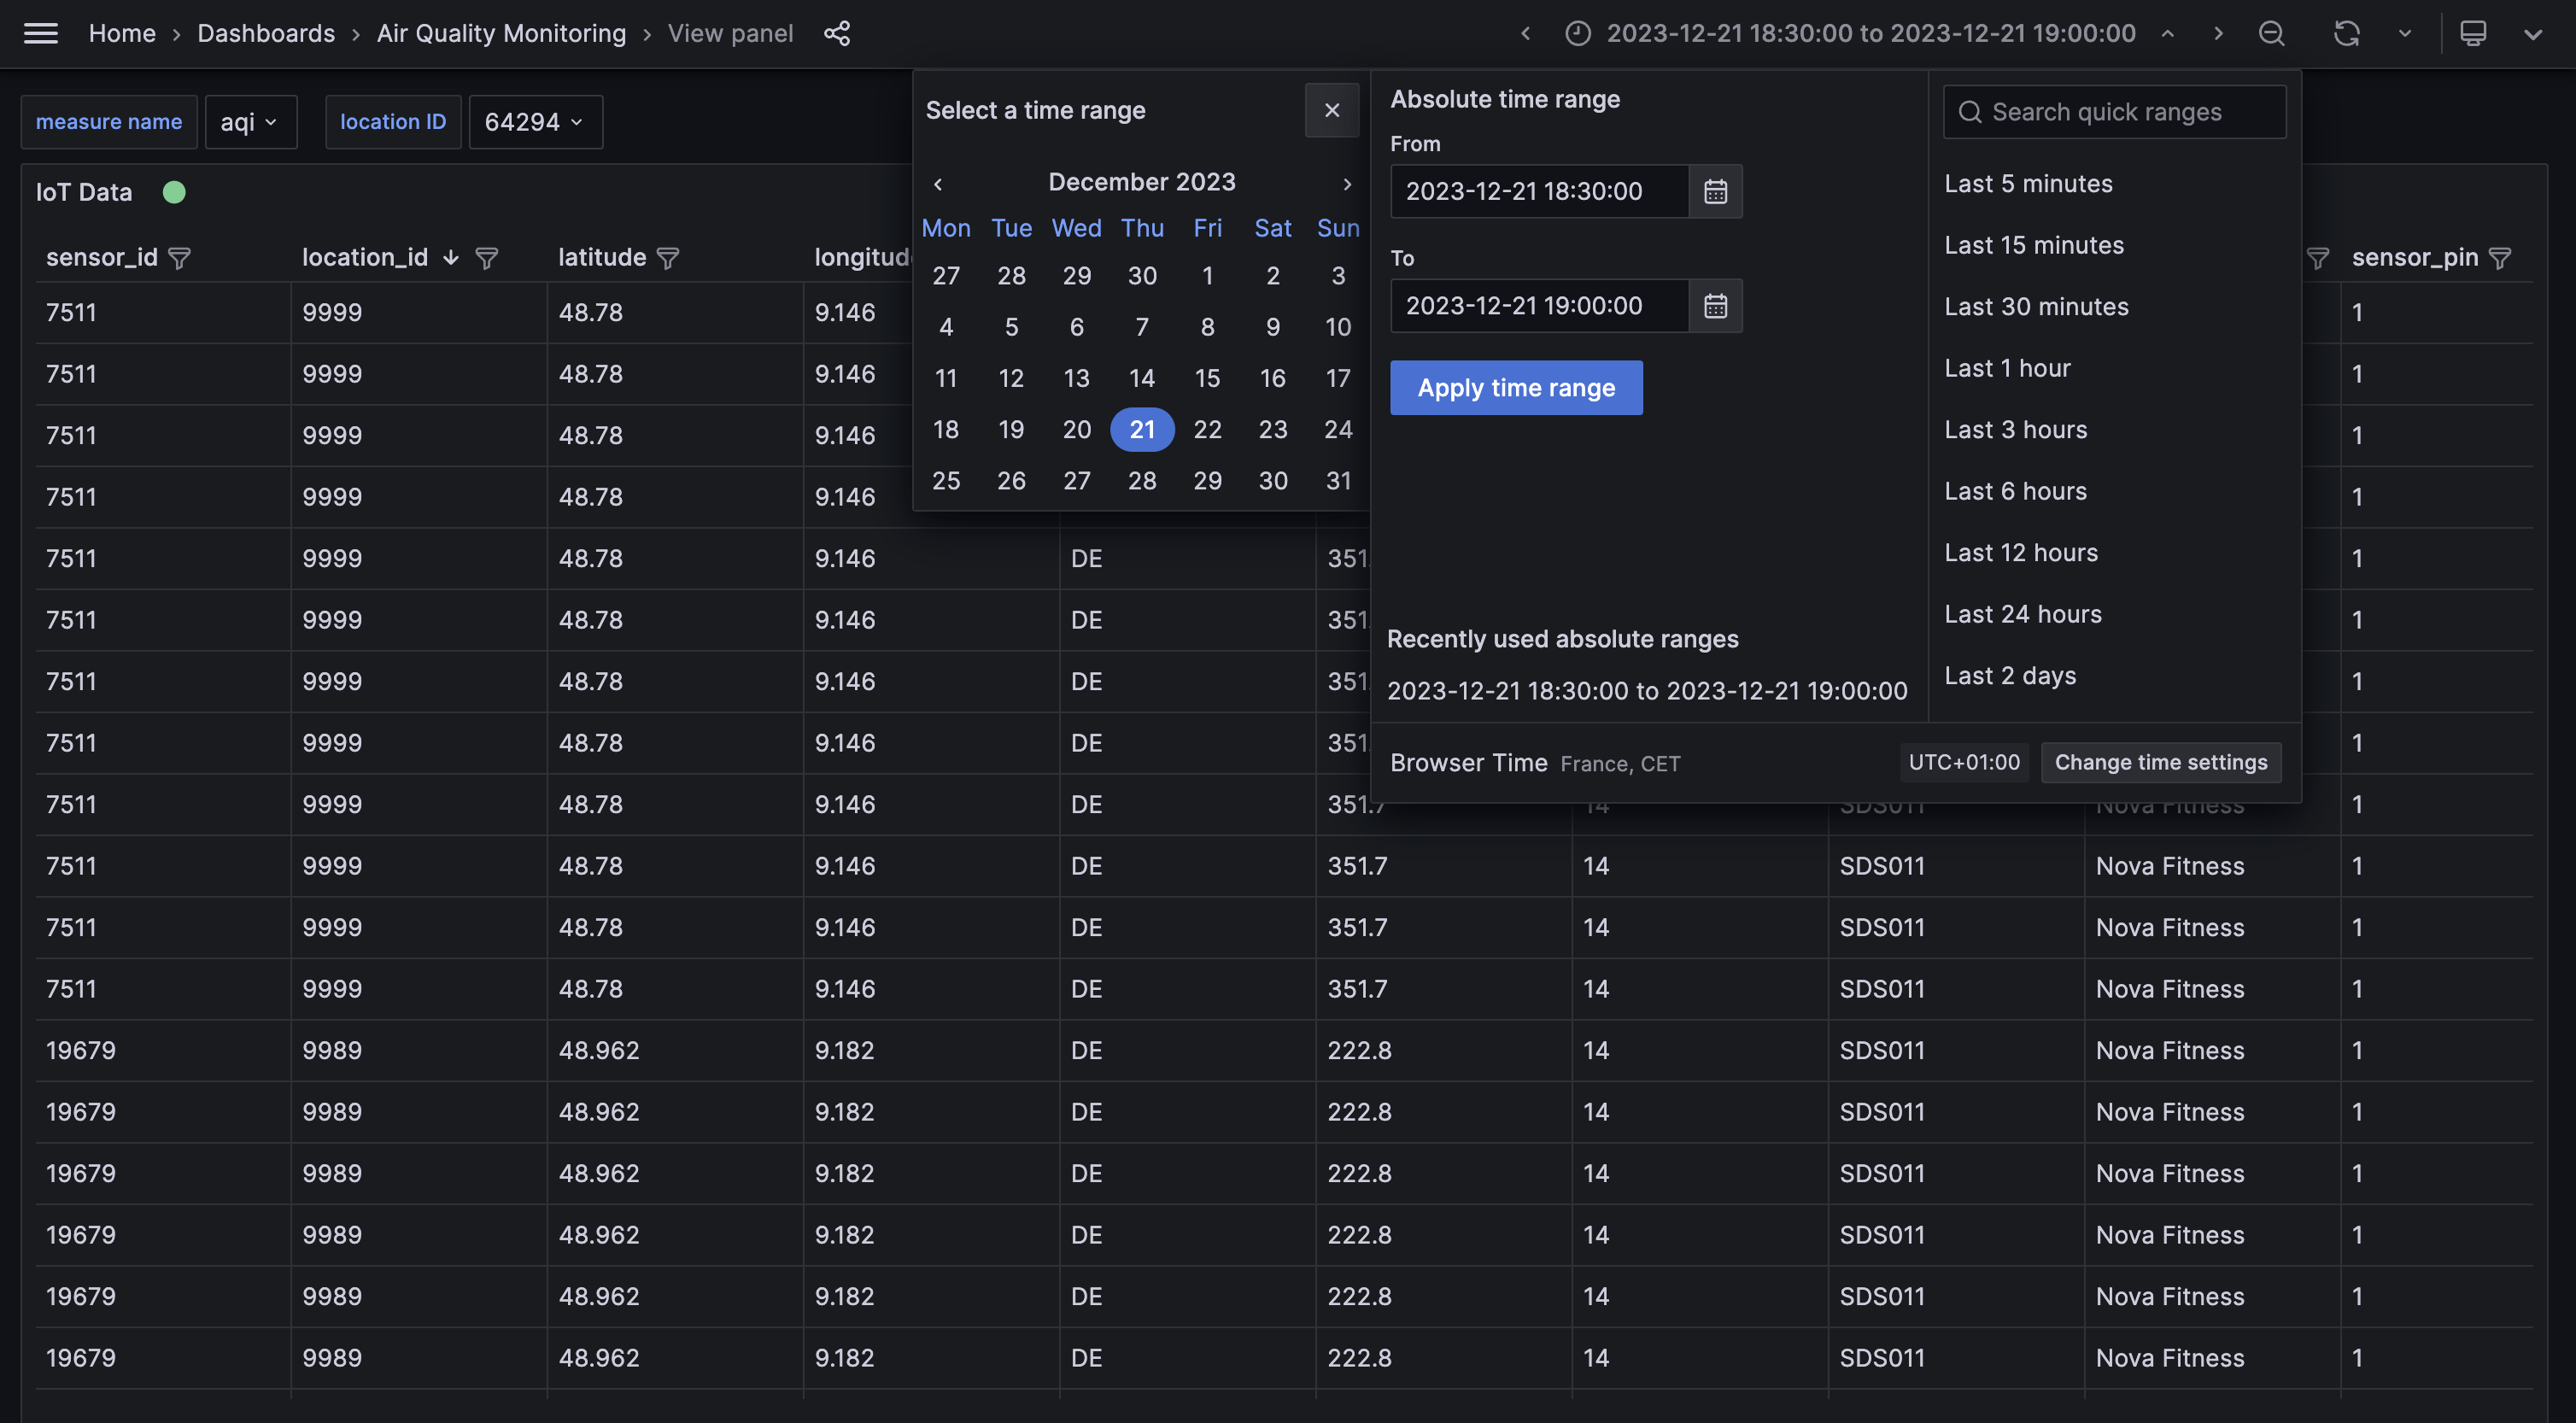
\includegraphics[width=1\linewidth]{images/time-range.png}
    \caption{Grafana Dashboard IoT Data Panel - Time Range Choice}\label{fig:grafana-iot-data-panel-time-range}
\end{figure}

\begin{figure}[H]
    \centering
    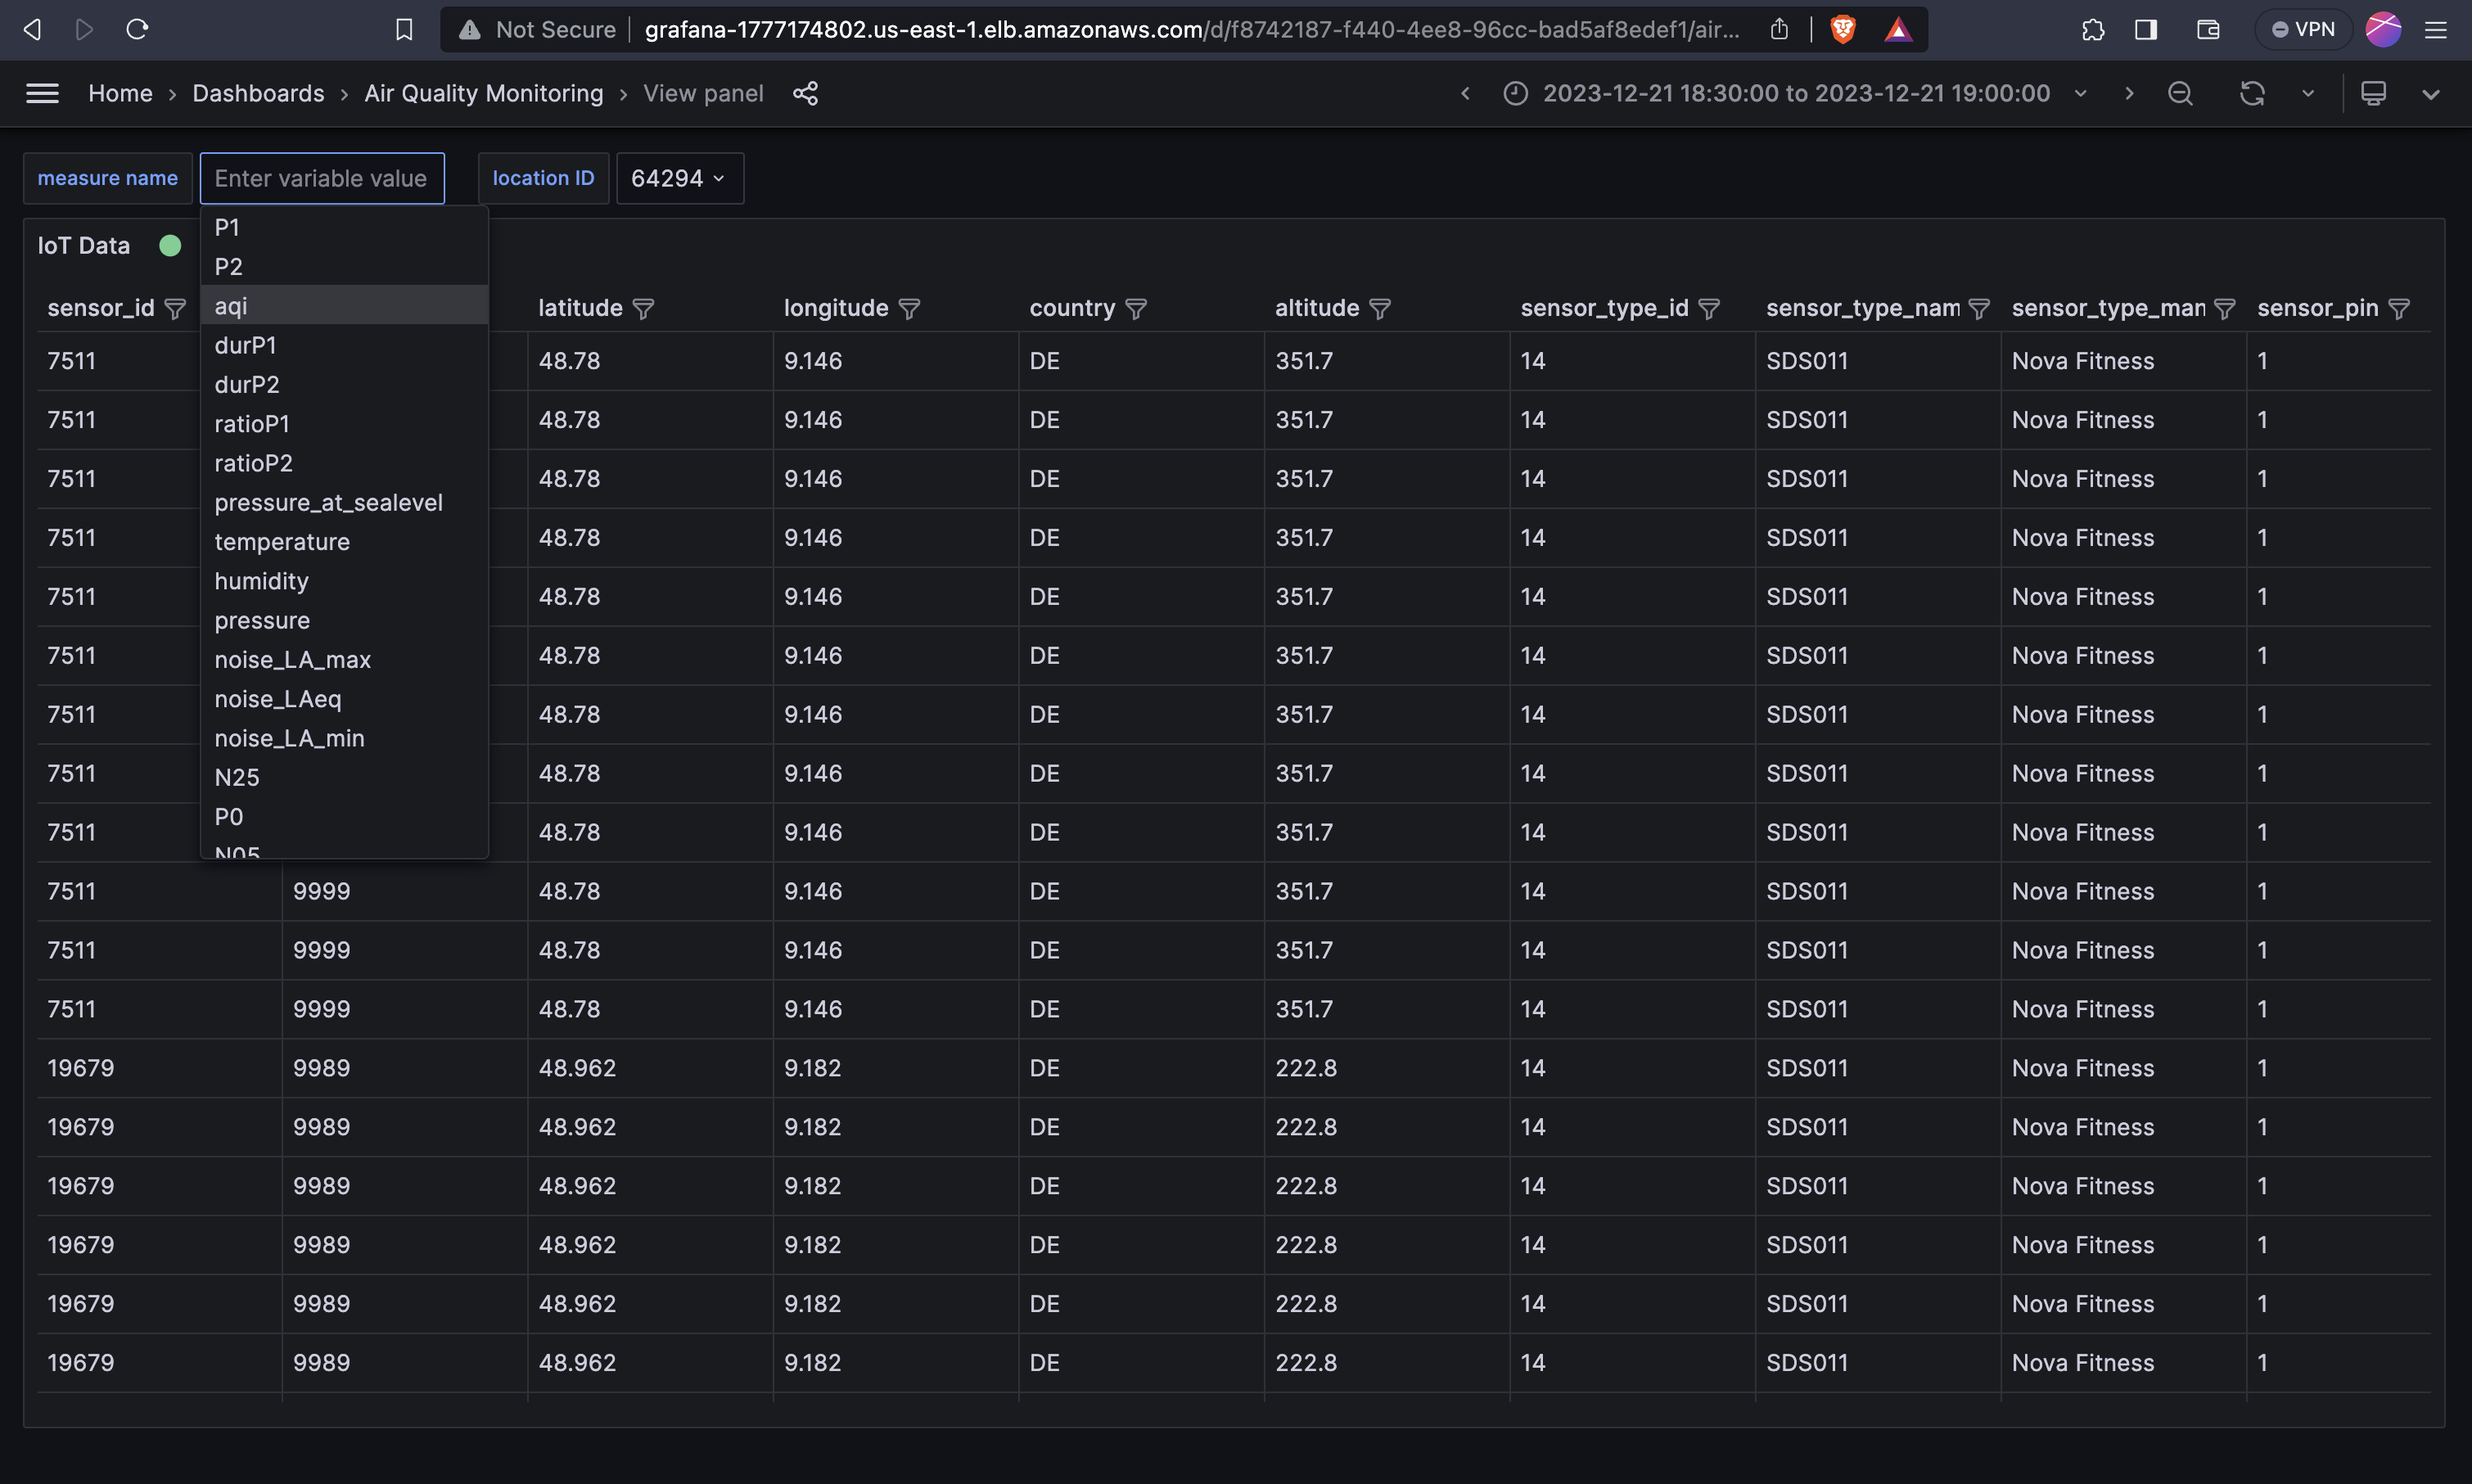
\includegraphics[width=1\linewidth]{images/measure-value.png}
    \caption{Grafana Dashboard IoT Data Panel - Measure Value Choice}\label{fig:grafana-iot-data-panel-measure-value}
\end{figure}

\begin{figure}[H]
    \centering
    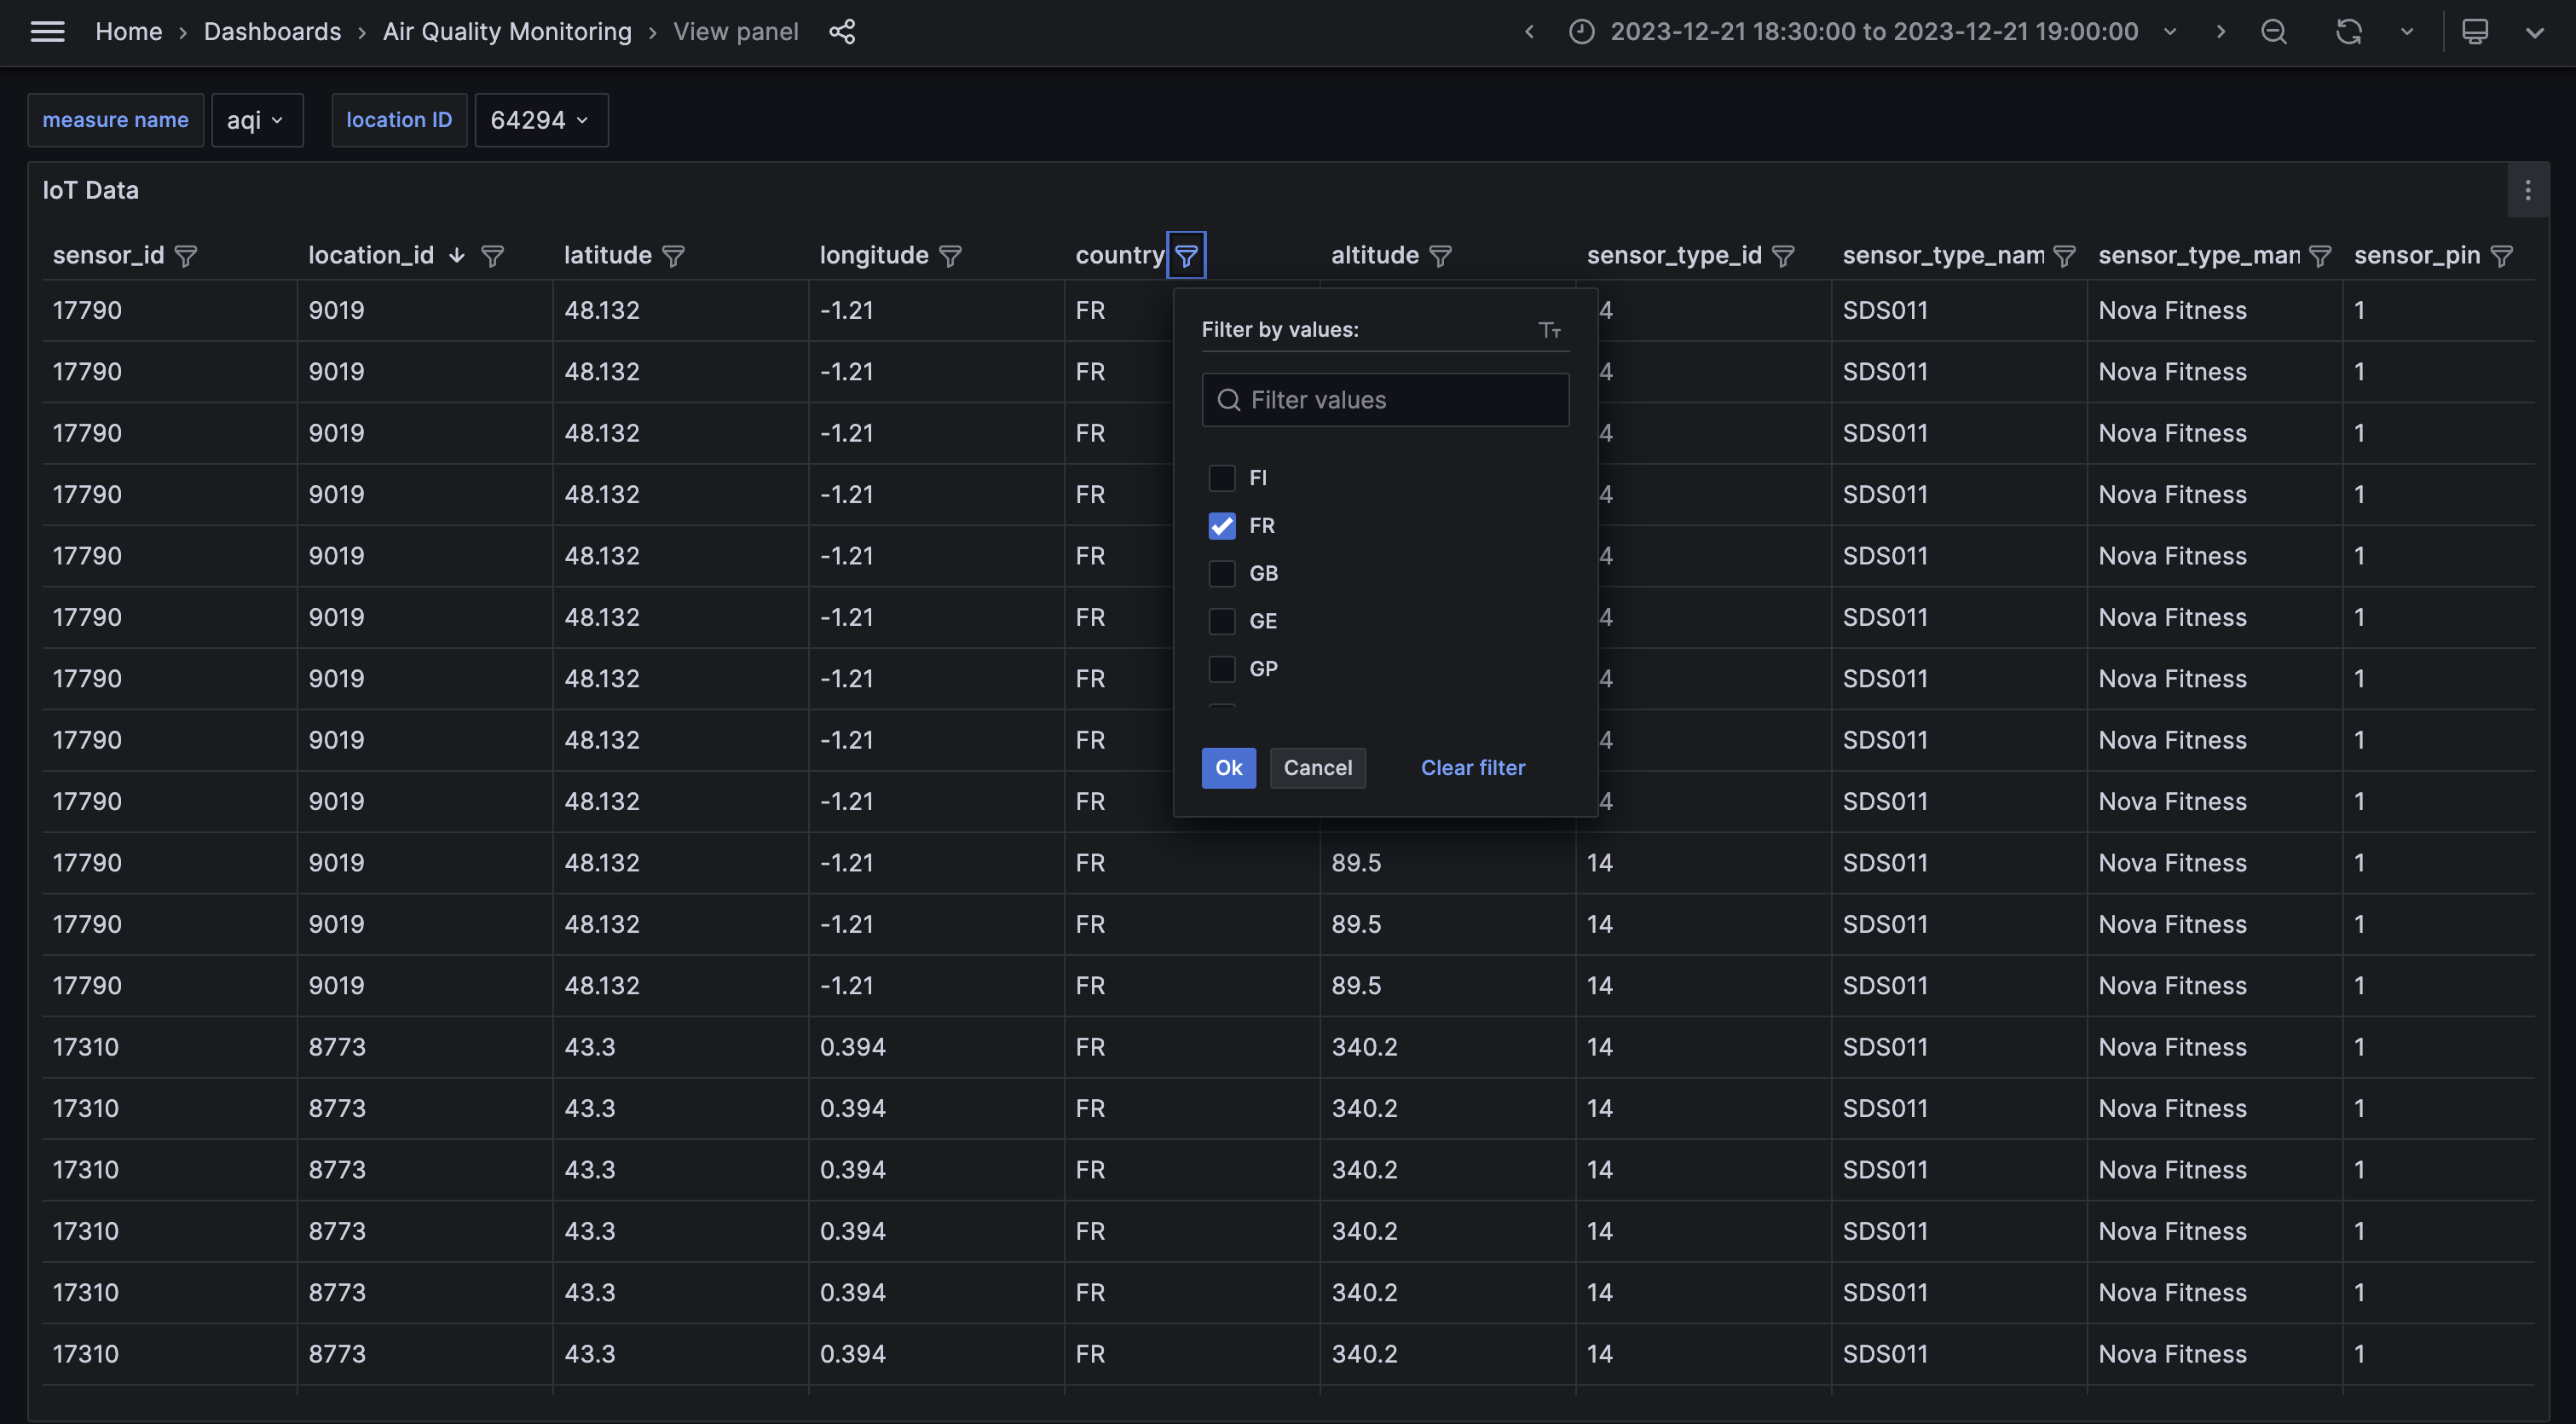
\includegraphics[width=1\linewidth]{images/filter.png}
    \caption{Grafana Dashboard IoT Data Panel - Apply a Filter}\label{fig:grafana-iot-data-panel-filter}
\end{figure}

\begin{figure}[H]
    \centering
    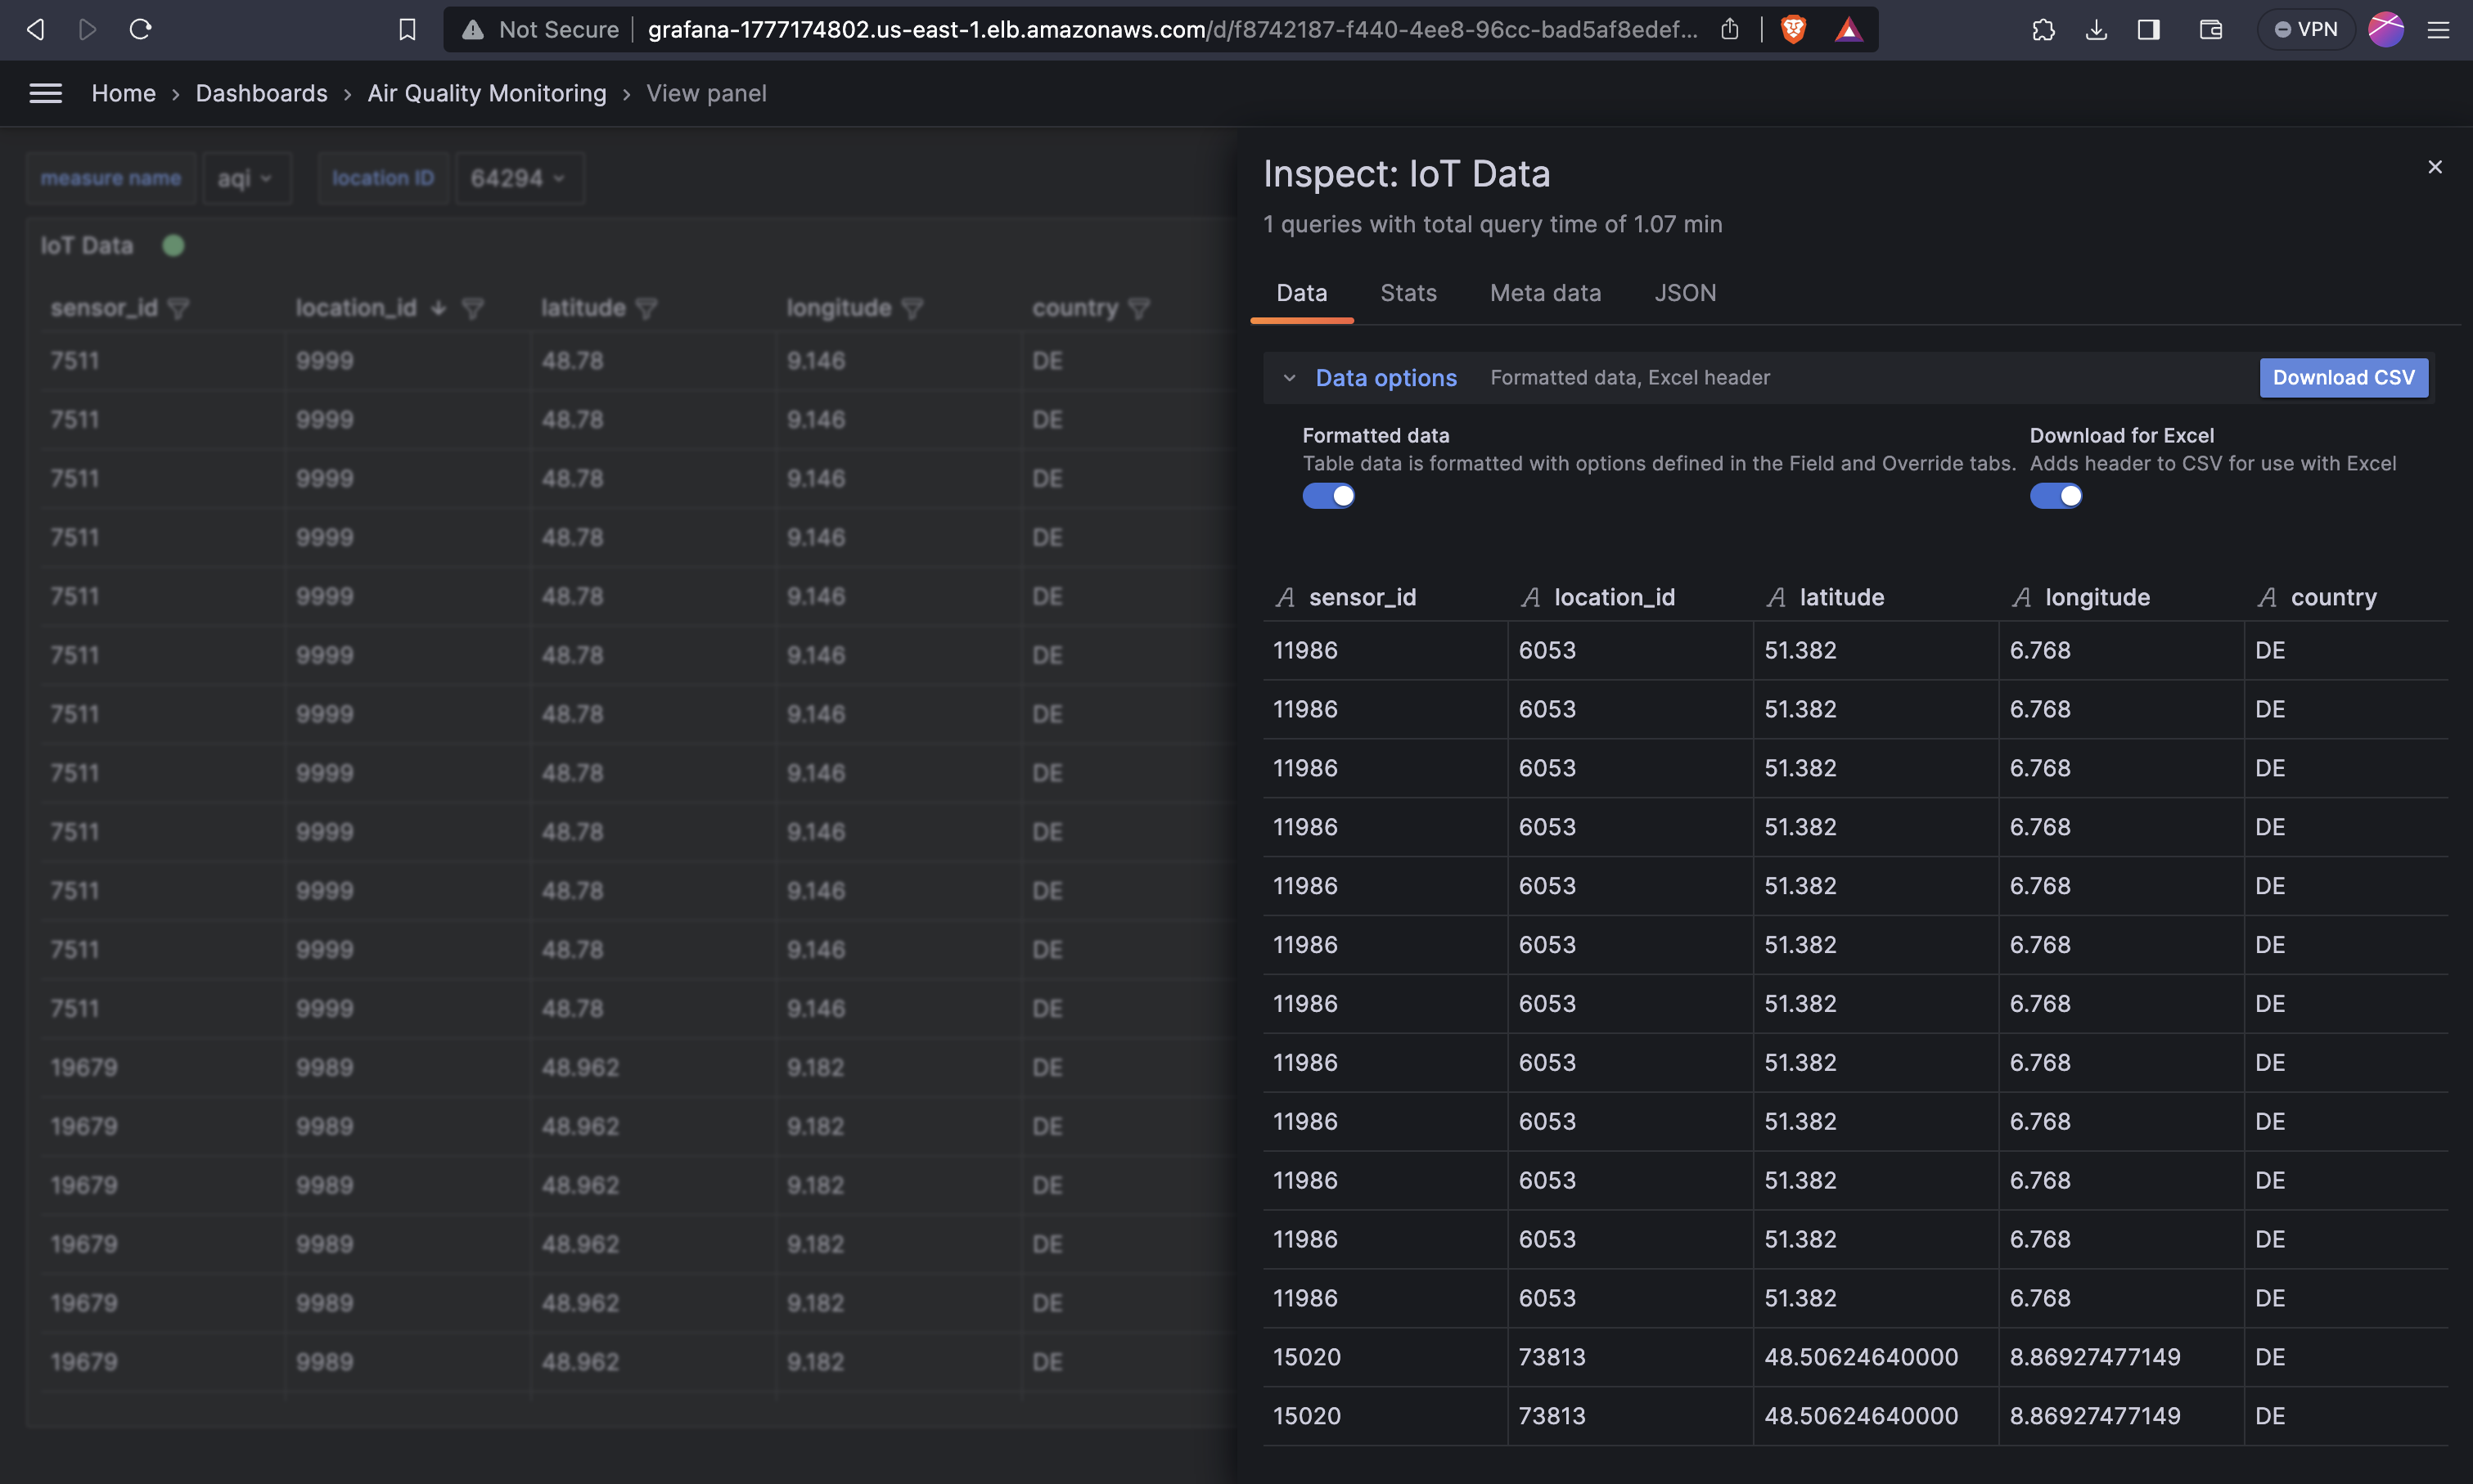
\includegraphics[width=1\linewidth]{images/export-2.png}
    \caption{Grafana Dashboard IoT Data Panel - Export Values}\label{fig:grafana-iot-data-panel-export}
\end{figure}

\newpage
\subsection{Load Test}
In order to test the scalability of the system, a load test was performed using
the Artillery load testing framework. The test consisted in simulating an
increasing number of customers consuming the grafana dashboards simultaneously,
to demonstrate the elasticity of the solution developed. The results of the
test are shown in Figure~\ref{fig:load-test-result}.

\begin{figure}[H]
    \centering
    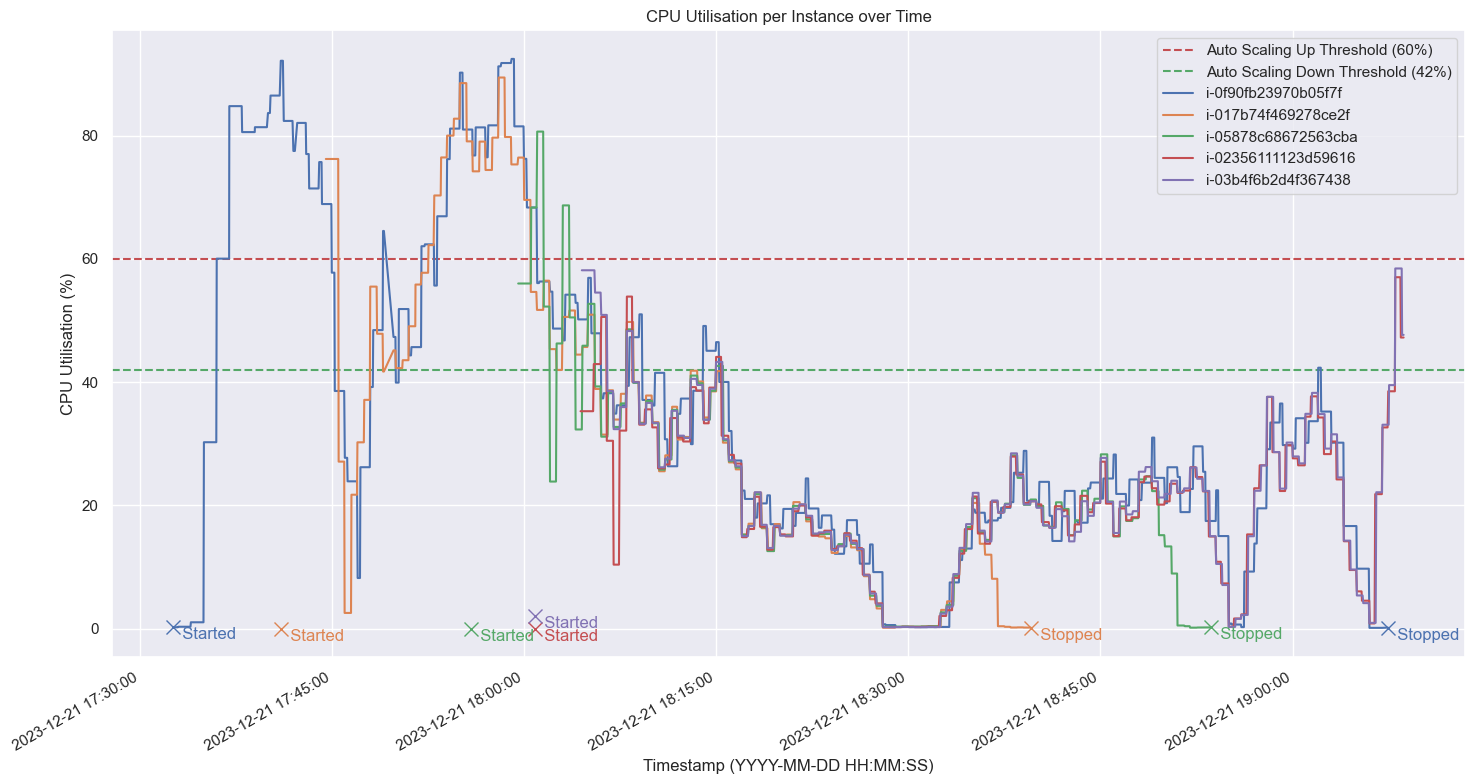
\includegraphics[width=1\linewidth]{images/autoscaling-test.png}
    \caption{Load Test Result}\label{fig:load-test-result}
\end{figure}

\newpage

\newpage
\section{Data Security and Sovereignty Considerations}
Data security and sovereignty are critical in the management of environmental
sensor data. Recent research trends in IoT security highlight the evolving
landscape of threats and protections in this field
\cite{CurrentResearchIoTSecurity2020}.

\subsection{Data Security}
In the realm of IoT, ensuring data security involves advanced encryption,
robust access control, and maintaining data integrity. The systematic mapping
study by \citeauthor{CurrentResearchIoTSecurity2020} provides insights into
current methodologies and research directions in IoT security, relevant to
environmental sensor data.

\subsection{Data Sovereignty}
Data sovereignty is influenced by varying international legislations, such as
GDPR, affecting data storage and cross-border data transfer. The study by
\citeauthor{CurrentResearchIoTSecurity2020} underscores the importance of
understanding these legal complexities in IoT environments.

\subsection{Specific Fields for Further Examination}
Areas needing heightened attention include personal data protection,
sensitivity of environmental data, and metadata security, as indicated by
recent IoT security research trends \cite{CurrentResearchIoTSecurity2020}.

Adhering to the latest security trends and regulatory frameworks is vital for
the ethical management of environmental sensor data. The evolving research in
IoT security serves as a guide for future developments in this field
\cite{CurrentResearchIoTSecurity2020}.

\newpage
\chapter{Conclusion}

In conclusion, this study presents a significant advancement in air quality
monitoring through IoT technologies, demonstrating the effectiveness of the
Grafana dashboard in data visualization and analysis. The successful load test
indicates the system's scalability, catering to simultaneous user access.
Addressing data security and sovereignty, the project highlights the importance
of robust data management practices in IoT environments. While acknowledging
certain limitations, this research lays a foundation for future explorations in
IoT security and data handling. Overall, it contributes valuable insights to
the field of environmental monitoring and data security, underscoring the
potential of IoT in addressing critical ecological issues.

\bibliographystyle{CranfieldNumbered}
\bibliography{CUCitations}

\appendix
\chapter{Documentation}

\begin{subappendices}
    \section{Project tree}
    \begin{lstlisting}[breaklines=true, basicstyle=\small]
    lib/
        collecting.py
        processing.py
        storing.py
    scripts/
        get_iam_credentials.sh
        start_spark_job.sh
    services/
        get_iam_credentials.service
        spark_python_job.service
        grafana_server.service
    test/
        artillery_load_test.yml
        monitoring.py
        metrics.csv
        results.json
        visualisation_load_test.ipynb
    main.py
    README.md
    requirements.txt
    \end{lstlisting}

    \section{Getting Started}
    To run the program, follow these steps:
    \begin{enumerate}
        \itemindent=17.87pt
        \item Create a virtual environment using \texttt{python3 -m venv venv}.
        \item Activate the virtual environment using \texttt{source venv/bin/activate}.
        \item Install the required dependencies using \texttt{pip3 install -r
                  requirements.txt}.
        \item Run the program using \texttt{python3 main.py}.
        \item Visualise the results using \texttt{visualisation.ipynb} (Jupyter Notebook).
    \end{enumerate}

    \section{Detailed Features of Functions}
    \begin{description}
        \item \texttt{collecting.py}
              \begin{itemize}
                  \item \texttt{fetch\_sensors\_data(sparkSession)}: Function to ingest the latest data from the sensors and returns it as a Spark DataFrame.
              \end{itemize}

        \item \texttt{processing.py}
              \begin{itemize}
                  \item \texttt{get\_aqi\_value\_p25(value)}: Function for calculating the AQI value for PM2.5.
                  \item \texttt{get\_aqi\_value\_p10(value)}: Function for calculating the AQI value for PM10.
                  \item \texttt{computeAQI(df)}: Function for calculating the AQI value for each particulate matter sensor and returning the DataFrame with the AQI column.
              \end{itemize}

        \item \texttt{storing.py}
              \begin{itemize}
                  \item \texttt{keepOnlyUpdatedRows(database\_name, table\_name, df)}: Function for keeping only the rows that have been updated in the DataFrame.
                  \item \texttt{\_print\_rejected\_records\_exceptions(err)}: Internal function for printing the rejected records exceptions.
                  \item \texttt{write\_records(database\_name, table\_name, client, records)}: Internal function for writing a batch of records to the Timestream database.
                  \item \texttt{writeToTimestream(database\_name, table\_name, partionned\_df)}: Function for writing the DataFrame to the Timestream database.
              \end{itemize}
    \end{description}
\end{subappendices}

\chapter{Source Codes}
\begin{subappendices}
    \section{Ingestion, Processing \& Storing Pipeline Source Code}
    \lstinputlisting[style=pythonstyle]{../main.py}\label{appendix:main}

    \newpage
    \section{Data Collecting Source Code}
    \lstinputlisting[style=pythonstyle]{../lib/collecting.py}\label{appendix:collecting}

    \newpage
    \section{Data Processing Source Code}
    \lstinputlisting[style=pythonstyle]{../lib/processing.py}\label{appendix:processing}

    \newpage
    \section{Data Storing Source Code}
    \lstinputlisting[style=pythonstyle]{../lib/storing.py}\label{appendix:storing}

    \newpage
    \section{Scripts \& Services Source Codes }
    \subsection{Scripts}

    Script used by the \texttt{get\_iam\_credentials} service to retrieve the IAM
    credentials from the metadata server.
    \lstinputlisting[style=bashstyle]{../scripts/get_iam_credentials.sh}\label{appendix:get-iam-credentials}

    Script used by the \texttt{spark\_python\_job} service to run the Python Spark
    job.\lstinputlisting[style=bashstyle]{../scripts/start_spark_job.sh}\label{appendix:start-spark-job}

    \newpage
    \subsection{Services}

    \subsubsection{Get IAM Credentials Service}
    Service used by the Ubuntu EC2 instance to retrieve the IAM credentials from
    the metadata server.
    \lstinputlisting[style=servicestyle]{../services/get_iam_credentials.service}\label{appendix:get-iam-credentials-service}

    \subsubsection{Spark Python Job Service}
    Service used by the Ubuntu EC2 instance to run the Python Spark job (Data
    Collecting, Processing and Storing).
    \lstinputlisting[style=servicestyle]{../services/spark_python_job.service}\label{appendix:spark-python-job-service}

    \newpage
    \subsubsection{Grafana Server Service}
    Service used by the Linux EC2 instances to run the Grafana server (Data
    Distributing).
    \lstinputlisting[style=servicestyle]{../services/grafana_server.service}\label{appendix:grafana-server-service}

    \newpage
    \section{Load Test Source Codes }

    \subsection{Artillery Load Test Configuration File}
    \lstinputlisting[style=ymlstyle]{../test/artillery_load_test.yml}\label{appendix:artillery-load-test}

    \newpage
    \subsection{Instances Monitoring Script}
    \lstinputlisting[style=pythonstyle]{../test/monitoring.py}\label{appendix:monitoring}
\end{subappendices}

\end{document}

